% A LaTeX template for MSc Thesis submissions to 
% Politecnico di Milano (PoliMi) - School of Industrial and Information Engineering
%
% S. Bonetti, A. Gruttadauria, G. Mescolini, A. Zingaro
% e-mail: template-tesi-ingind@polimi.it
%
% Last Revision: October 2021
%
% Copyright 2021 Politecnico di Milano, Italy. NC-BY

\documentclass{Configuration_Files/PoliMi3i_thesis}

%------------------------------------------------------------------------------
%	REQUIRED PACKAGES AND  CONFIGURATIONS
%------------------------------------------------------------------------------

% CONFIGURATIONS
\usepackage{parskip} % For paragraph layout
\usepackage{setspace} % For using single or double spacing
\usepackage{emptypage} % To insert empty pages
\usepackage{multicol} % To write in multiple columns (executive summary)
\setlength\columnsep{15pt} % Column separation in executive summary
\setlength\parindent{0pt} % Indentation
\raggedbottom  

% PACKAGES FOR TITLES
\usepackage{titlesec}
% \titlespacing{\section}{left spacing}{before spacing}{after spacing}
\titlespacing{\section}{0pt}{3.3ex}{2ex}
\titlespacing{\subsection}{0pt}{3.3ex}{1.65ex}
\titlespacing{\subsubsection}{0pt}{3.3ex}{1ex}
\usepackage{color}

% PACKAGES FOR LANGUAGE AND FONT
\usepackage[english]{babel} % The document is in English  
\usepackage[utf8]{inputenc} % UTF8 encoding
\usepackage[T1]{fontenc} % Font encoding
\usepackage[11pt]{moresize} % Big fonts

% PACKAGES FOR IMAGES
\usepackage{graphicx}
\usepackage{transparent} % Enables transparent images
\usepackage{eso-pic} % For the background picture on the title page
\usepackage{subcaption} % Numbered and caption subfigures using \subfloat.
\usepackage{tikz} % A package for high-quality hand-made figures.
\usetikzlibrary{}
\graphicspath{{./Images/}} % Directory of the images
\usepackage{caption} % Coloured captions
\usepackage{xcolor} % Coloured captions
\usepackage{amsthm,thmtools,xcolor} % Coloured "Theorem"
\usepackage{float}

% STANDARD MATH PACKAGES
\usepackage{amsmath}
\usepackage{amsthm}
\usepackage{amssymb}
\usepackage{amsfonts}
\usepackage{bm}
\usepackage[overload]{empheq} % For braced-style systems of equations.
\usepackage{fix-cm} % To override original LaTeX restrictions on sizes

% PACKAGES FOR TABLES
\usepackage{tabularx}
\usepackage{longtable} % Tables that can span several pages
\usepackage{colortbl}

% PACKAGES FOR ALGORITHMS (PSEUDO-CODE)
\usepackage{algorithm}
\usepackage{algorithmic}

% PACKAGES FOR REFERENCES & BIBLIOGRAPHY
\usepackage[colorlinks=true,linkcolor=black,anchorcolor=black,citecolor=black,filecolor=black,menucolor=black,runcolor=black,urlcolor=black]{hyperref} % Adds clickable links at references
\usepackage{cleveref}
\usepackage[square, numbers, sort&compress]{natbib} % Square brackets, citing references with numbers, citations sorted by appearance in the text and compressed
\bibliographystyle{abbrvnat} % You may use a different style adapted to your field

% OTHER PACKAGES
\usepackage{pdfpages} % To include a pdf file
\usepackage{afterpage}
\usepackage{lipsum} % DUMMY PACKAGE
\usepackage{fancyhdr} % For the headers
\fancyhf{}

% Input of configuration file. Do not change config.tex file unless you really know what you are doing. 
% Configuration package
\usepackage[bottom=2.0cm,top=2.0cm,left=2.0cm,right=2.0cm]{geometry}
\raggedbottom 

% Create color bluePoli (-> manuale grafica coordinata:  https://www.polimi.it/fileadmin/user_upload/il_Politecnico/grafica-coordinata/2015_05_11_46xy_manuale_grafica_coordinata.pdf)
\definecolor{bluePoli}{cmyk}{0.4,0.1,0,0.4}

% Custom theorem environments
\declaretheoremstyle[
  headfont=\color{bluePoli}\normalfont\bfseries,
  bodyfont=\color{black}\normalfont\itshape,
]{colored}

\captionsetup[figure]{labelfont={color=bluePoli}} % Set colour of the captions
\captionsetup[table]{labelfont={color=bluePoli}} % Set colour of the captions
\captionsetup[algorithm]{labelfont={color=bluePoli}} % Set colour of the captions

\theoremstyle{colored}
\newtheorem{theorem}{Theorem}[section]
\newtheorem{proposition}{Proposition}[section]

% Enhances the features of the standard "table" and "tabular" environments.
\newcommand\T{\rule{0pt}{2.6ex}}
\newcommand\B{\rule[-1.2ex]{0pt}{0pt}}

% Algorithm description
\newcounter{algsubstate}
\renewcommand{\thealgsubstate}{\alph{algsubstate}}
\newenvironment{algsubstates}{
    \setcounter{algsubstate}{0}%
    \renewcommand{\STATE}{%
    \stepcounter{algsubstate}%
    \Statex {\small\thealgsubstate:}\space}
    }{}
    
% Custom theorem environment
\newcolumntype{L}[1]{>{\raggedright\let\newline\\\arraybackslash\hspace{0pt}}m{#1}}
\newcolumntype{C}[1]{>{\centering\let\newline\\\arraybackslash\hspace{0pt}}m{#1}}
\newcolumntype{R}[1]{>{\raggedleft\let\newline\\\arraybackslash\hspace{0pt}}m{#1}}

% Custom itemize environment
\setlist[itemize,1]{label=$\bullet$}
\setlist[itemize,2]{label=$\circ$}
\setlist[itemize,3]{label=$-$}
\setlist{nosep}

% Create command for background pic
\newcommand\BackgroundPic{% Adding background picture
	\put(237,365){
	    \parbox[b][\paperheight]{\paperwidth}{%
	    \vfill
		\centering
		\transparent{0.4}
		
\includegraphics[width=0.44\paperwidth]{raggiera_polimi.eps}%
		\vfill}
		}
}

% Set indentation
\setlength\parindent{0pt}

% Custom title commands
\titleformat{\section}
{\color{bluePoli}\normalfont\Large\bfseries}
{\color{bluePoli}\thesection.}{1em}{}
\titlespacing*{\section}
{0pt}{3.3ex}{3.3ex}

\titleformat{\subsection}
{\color{bluePoli}\normalfont\large\bfseries}
{\color{bluePoli}\thesubsection.}{1em}{}
\titlespacing*{\subsection}
{0pt}{3.3ex}{3.3ex}

% Custom headers and footers
\pagestyle{fancy}
\fancyhf{}
      
\fancyfoot{}
\fancyfoot[C]{\thepage} % page
\renewcommand{\headrulewidth}{0mm} % headrule width
\renewcommand{\footrulewidth}{0mm} % footrule width

\makeatletter
\patchcmd{\headrule}{\hrule}{\color{black}\hrule}{}{} % headrule
\patchcmd{\footrule}{\hrule}{\color{black}\hrule}{}{} % footrule
\makeatother

%----------------------------------------------------------------------------
%	NEW COMMANDS DEFINED
%----------------------------------------------------------------------------


%----------------------------------------------------------------------------
%	ADD YOUR PACKAGES (be careful of package interaction)
%----------------------------------------------------------------------------

%----------------------------------------------------------------------------
%	ADD YOUR DEFINITIONS AND COMMANDS (be careful of existing commands)
%----------------------------------------------------------------------------

%----------------------------------------------------------------------------
%	BEGIN OF YOUR DOCUMENT
%----------------------------------------------------------------------------

\begin{document}

\fancypagestyle{plain}{%
\fancyhf{} % Clear all header and footer fields
\fancyhead[RO,RE]{\thepage} %RO=right odd, RE=right even
\renewcommand{\headrulewidth}{0pt}
\renewcommand{\footrulewidth}{0pt}}

%----------------------------------------------------------------------------
%	TITLE PAGE
%----------------------------------------------------------------------------

\pagestyle{empty} % No page numbers
\frontmatter % Use roman page numbering style (i, ii, iii, iv...) for the preamble pages

\puttitle{
	title=Evolutionary-based procedural\\content generation for First\\Person Shooters in Unity, % Title of the thesis
	name=Simone Bari, % Author Name and Surname
	course=Computer Science and Engineering - Ingegneria \mbox{Informatica}, % Study Programme (in Italian)
	ID  = 944517,  % Student ID number (numero di matricola)
	advisor= Prof. Daniele Loiacono, % Supervisor name
	coadvisor=Prof. Pier Luca Lanzi, % Co-Supervisor name, remove this line if there is none
	academicyear={2021-22},  % Academic Year
} % These info will be put into your Title page 

%----------------------------------------------------------------------------
%	PREAMBLE PAGES: ABSTRACT (inglese e italiano), EXECUTIVE SUMMARY
%----------------------------------------------------------------------------
\startpreamble
\setcounter{page}{1} % Set page counter to 1

% ABSTRACT IN ENGLISH
\chapter*{Abstract} 
\textit{Level design} plays a fundamental role in the development of a video game and is one of the components that most influences its final quality. However, there is currently a lack of discipline for this task, and often \textit{level design} is seen more as an art to be entrusted to experience and common sense, without a more accurate scientific investigation.

In recent years, the academic world has begun to take its first timid steps towards studying this field, but there is still a lack of common vocabularies and standard techniques and tools to evaluate and test theories, especially in the context of first-person shooters.

An attempt to introduce an open-source tool that would address this problem was made by Ballabio, who introduced a modern open-source framework in \textit{Unity} that represents a skeleton of an FPS. However, this framework has a serious flaw in the lack of bots that allow the simulation of various matches and the subsequent extraction of observed gameplay dynamics.

In our work, we wanted to overcome this limitation by designing and developing a relatively simple and flexible bot system, in order to be able exploit the capabilities of procedural content generation with search algorithms, already tested in various other studies, using the framework.

After having introduced bots, we wanted to test a novel approach to map representation based on graphs, comparing the results obtained from various genetic evolutions using this representation with another more well-known and widespread representation.

% Here goes the Abstract in English of your thesis followed by a list of keywords.
% The Abstract is a concise summary of the content of the thesis (single page of text) and a guide to the most important contributions included in your thesis.
% The Abstract is the very last thing you write.
% It should be a self-contained text and should be clear to someone who hasn't (yet) read the whole manuscript.
% The Abstract should contain the answers to the main scientific questions that have been addressed in your thesis.
% It needs to summarize the adopted motivations and the adopted methodological approach as well as the findings of your work and their relevance and impact.
% The Abstract is the part appearing in the record of your thesis inside POLITesi, the Digital Archive of PhD and Master Theses (Laurea Magistrale) of Politecnico di Milano.
% The Abstract will be followed by a list of four to six keywords.
% Keywords are a tool to help indexers and search engines to find relevant documents. To be relevant and effective, keywords must be chosen carefully. They should represent the content of your work and be specific to your field or sub-field. Keywords may be a single word or two to four words. 

\textbf{Keywords:} \textit{Level design}, videogame bots, procedural content generation, graph theory. % Keywords

% ABSTRACT IN ITALIAN
\chapter*{Abstract in lingua italiana}
Il \textit{level design} è un aspetto fondamentale nello sviluppo di un videogioco e rappresenta una delle componenti che maggiormente influenzano la qualità finale del prodotto. Tuttavia, attualmente non esiste una disciplina consolidata per tale attività e spesso il level design viene considerato come un'arte da affidare all'esperienza e al buon senso, senza che venga applicato un approccio scientifico più rigoroso.

Negli ultimi anni, il mondo accademico ha iniziato a esplorare questa area di ricerca, ma ancora mancano vocabolari comuni, tecniche e strumenti standard per valutare le teorie e testarle, soprattutto nel contesto degli sparatutto in prima persona.

Un tentativo di ovviare a questa mancanza è stato fatto da Ballabio, che ha introdotto un moderno framework open-source in \textit{Unity} che rappresenta uno scheletro di un FPS. Tuttavia, il framework presenta una grave carenza nella mancanza di bot per la simulazione di partite e l'estrazione delle dinamiche di gioco osservate.

Nel nostro lavoro, abbiamo voluto colmare questa lacuna progettando e sviluppando un sistema di bot relativamente semplice e flessibile, in modo da poter sfruttare le capacità della generazione procedurale di contenuti con algoritmi di ricerca, già testati in altre ricerche, direttamente usando il Framework.

Una volta introdotto i bot, abbiamo infine voluto testare un innovativo approccio alla rappresentazione di mappe basato sui grafi, confrontando i risultati ottenuti dalle evoluzioni genetiche che utilizzano tale rappresentazione con quelli di una rappresentazione più diffusa e conosciuta.

\textbf{Parole chiave:} \textit{Level design}, bot per videogiochi, generazione procedurale di contenuti, teoria dei grafi.   % Keywords (italian)

%----------------------------------------------------------------------------
%	LIST OF CONTENTS/FIGURES/TABLES/SYMBOLS
%----------------------------------------------------------------------------

% TABLE OF CONTENTS
\thispagestyle{empty}
\tableofcontents % Table of contents 
\thispagestyle{empty}
\cleardoublepage

% LIST OF FIGURES
\listoffigures

% LIST OF TABLES
%\listoftables

% LIST OF SYMBOLS
% Write out the List of Symbols in this page


%-------------------------------------------------------------------------
%	THESIS MAIN TEXT
%-------------------------------------------------------------------------

\addtocontents{toc}{\vspace{2em}} % Add a gap in the Contents, for aesthetics
\mainmatter % Begin numeric (1,2,3...) page numbering

% --------------------------------------------------------------------------
% NUMBERED CHAPTERS % Regular chapters following
% --------------------------------------------------------------------------

\chapter{Introduction}

The development of video games is a complex process and the most relevant aspect, in addition to graphics and narrative, is undoubtedly \textit{gameplay}, which refers to the ways in which the player interacts with the game. The definition of a game's \textit{gameplay} is given by a set of rules, the \textit{game design}, which is presented to the user tangibly through the worlds in which the game takes place and the set of mechanics available to the player to interact with the world. The combination of these two elements, known as \textbf{level design}, plays a fundamental role in defining the overall gaming experience.

In this work, we will focus on analyzing the theory of \textit{level design} in \textbf{First-Person Shooter} (FPS) video games, one of the most popular and well-known video game genres, particularly in the context of competitive shooters. In such games, in addition to considering the greater immersion required by the game world due to the first-person view, it is necessary to pay particular attention to the careful balancing of gameplay mechanics and interactions between various play styles during matches in order to ensure enjoyable and interesting gaming experiences.

Despite the importance of level design in FPS games, the topic has been little explored in the scientific field, with a lack of specific standards and vocabulary. In many cases, the success of a level design depends solely on the designer's experience and personal techniques, without a true understanding of the reasons behind their functioning.

Only recently have academic environments begun to pay greater attention to the identification, definition, and understanding of various design patterns and techniques in order to develop new tools useful for level design. Among the analyzed techniques, the use of evolutionary algorithms for procedural map generation seems particularly interesting, considering their effectiveness in other fields of application.

However, the use of evolutionary algorithms requires the availability of game data to guide the search for such procedures. To obtain this data, it is possible to involve human players or use bots for match simulation. In this thesis, we have decided to integrate an artificial intelligence system for match simulation through bots to the open-source Framework developed by Ballabio in \cite{ballabio_framework}. 

We then leveraged these bots to test a new type of map encoding using evolutionary algorithm.

\section{Contents of the thesis}
This work is structured in the following way:

In the second chapter we provide an overview of the current state of the art for what concerns \textit{level design} and \textit{procedural content generation} with \textit{evolutionary algorithms} applied to FPS games. We then briefly describe balancing in video games and FPS.

In the third chapter we describe bots for video games, focusing on their purpose, their artificial intelligence model and some techniques to implement their decision making capabilities.

In the fourth chapter we describe the Ballabio Unity framework, starting with a brief overview of what it offers to then focus on the bot system we added for this thesis.

In the fifth chapter, after verifing how different bot profiles compare to the others, we leverage the Framework and the newly developed bots to test evolution of new maps using old and new map representations.

Finally, in the conclusion we sum up the work we have done, the results we obtained and the issues and limitations we faced.

Additionally, in Appendix A, we show the syntax used in this thesis to represent the behaviour trees used to model the decision making processes of our bots.

\section{Contribution of this thesis}
In this thesis, we have designed, implemented, and tested a new open-source bot system for first-person shooter games in Unity. Despite its rich set of features and tools, Unity does not provide any out-of-the-box solutions for bot development.

Using these bots, we have introduced a new genome for encoding maps, called \textit{Grid-graph}. \textit{Grid-graph} builds upon key concepts, such as \textit{Rooms} and \textit{Corridors}, used by its predecessors while addressing some of their limitations. We have then evaluated the use of \textit{Grid-graph} in evolving balanced 1v1 maps for games which feature an unbalance in the skill level of players, and compared its performance with the \textit{All-black} representation first introduced by Cardamone \cite{cardamone_evolving_maps}.

\chapter{State of the art}

In this chapter we introduce the theory of level design; we examine how the problem is being tackled for singleplayer and multiplayer first person shooters both by the industry and the academical research. \\
We then proceed to analyze \textit{Procedural Content Generation} (PCG) and, specifically, \textit{Search-Based Procedural Content Generation} (SB-PCG) to generate and evaluate new content and, specifically, new maps for videogames, focusing on the research for FPS. \\
Lastly, we consider the concept of video game difficulty, with a particular focus on how multiplayer games and how maps can affect it. \\

\section{Level design theory}

\textit{Level design} is the discipline concerned with the creation of video game levels. Starting from a game concept, the level designer is tasked to build environments that explore the game concept by proposing challenges to the player. In this sense, the level designer is the one that transforms the simple game idea into something tangible.

\textit{Level design} is a fundamental task in the development of a game and it’s now extremely common to have figures specialized in this function. However, level design is not a well defined process yet: due to the level of imagination, trial and error and user input requested, it’s not easy to understand what the fundamental steps to achieve a good level design are \cite{the_invisible_hand}. 

In the years there have been researches aimed at finding common strategies to tackle level design, but often those researches are quite limited in scope since they consider a single genre of game (and often not covering it completely) and tend to get obsolete quickly due to the fast evolution of game and the introduction of new dynamics. Consider for example a game like Fortnite\footnote{People Can Fly, 2017}, a third person shooter which uniquely allows players to build structures that can be used as covers or look-out point. The introduction of a single dynamic (altering the map topology) completely changes the way level design has to be tackled, potentially invalidating other techniques used for other, more traditional third person shooters.

Despite this, there are some core ideas and techniques behind level design which remain valid no matter what, such as the level flow. In single player and cooperative multiplayer games, the level flow is defined as the series of action and movements that the player needs to perform to complete a level. The quality of a level flow can be measured in different ways, for example by checking whether the players ever felt lost or overwhelmed or by measuring how often the various game dynamics are used in a satisfying way.
There are various ways to guide the user according to the level flow: sound, architecture, items, collectibles, lightning, illumination, color coded conventions are all examples of resources that a level designer can use to guide the user along the correct path. 

\begin{figure}[hbpt]
\centering
  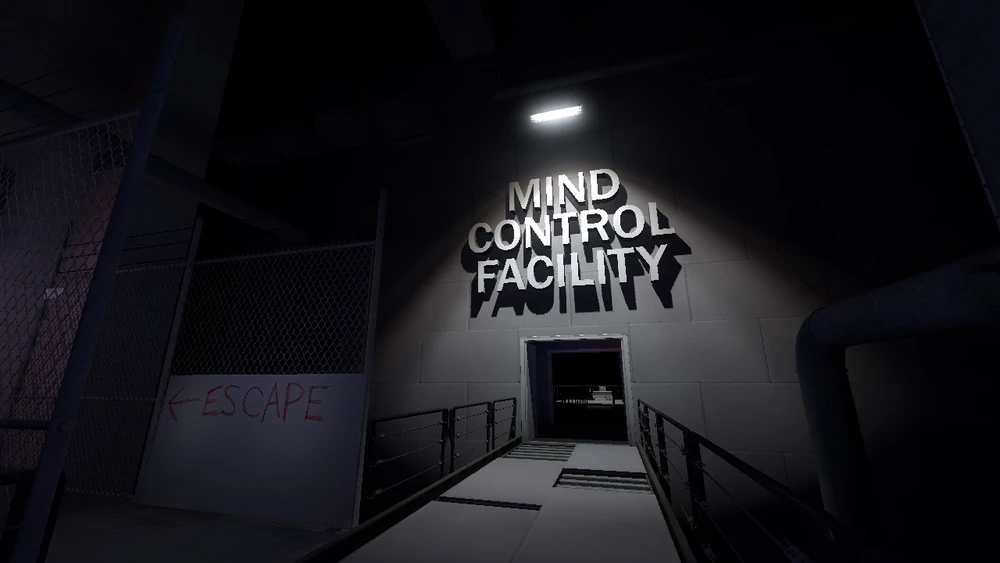
\includegraphics[width=0.8\linewidth]{Images/images/stanley_parable.png}
  \caption[Usage of lighting is The Stanley Parable]{In this section of \textit{The Stanley parable}\footnotemark, a game known for playing with and deconstructing common gaming tropes, lighting is used to great effect to guide them through the \textit{Mind Control Facility} room, distracting them from the "Escape" path marked on the left.}
  \label{fig:stanley_parable}
\end{figure}
\footnotetext{Galactic Cafe, 2013}

A brilliant example of this is Mirror’s Edge \footnote{Digital Illusions CE, 2008.
}, which uses a really clear color code, with red highlighting interactable objects in an otherwise white world, to guide the player through its fast-paced levels. There are also even more inventive solutions, like the dynamic flock of birds in Half-Life 2\footnote{Valve, 2004.}, used to catch the player attention or to warn him of incoming dangers \cite{half_life_2}.

% Finally, sounds and architectures are other elements that can be used to guide the player. In the academic environment, a lot of researchers have analyzed the effectiveness of this kind of solutions: Alotto[4] considers how architecture influences the decisions of the player, whereas Hoeg[5] also considers the effect of sounds, objects and illumination, with the last being the focus of Brownmiller’s[6] work. %In competitive multiplayer games the level flow is defined by how the players interact with each other and with the environment. Given that the objective is no longer to complete a level but to beat the opponents, in this kind of games there is no specific path to guide the player to, so the influence that the level designer can exert is much more limited and most of the control comes from the map design and the placement of elements. Güttler et al [Christian Güttler e Troels Degn Johansson. ‘Spatial Principles of Level design in Multi-player First-person Shooters’]. studied spatial design and gameplay evolution of various multiplayer maps and identified what they call “collision points”, the spots where the majority of conflicts occur. By carefully placing spawn points and collectible and designing the connectivity of the map (e.g. choke points and open areas), a level designer can partially control where this collision points will occur, thus influencing the level flow.

In competitive multiplayer games the level flow is defined by how the players interact with each other and with the environment. Given that the objective is no longer to complete a level but to beat the opponents, in this kind of games there is no specific path to guide the player to, so the influence that the level designer can exert is much more limited and most of the control comes from the map design and the placement of elements. Güttler et al \cite{spatial_principles_level_design} studied spatial design and gameplay evolution of various multiplayer maps and identified what they call “collision points”, the spots where the majority of conflicts occur. By carefully placing spawn points and collectible and designing the connectivity of the map (e.g. choke points and open areas), a level designer can partially control where this collision points will occur, thus influencing the level flow. 

In the academic world, level flow for single and multiplayer games has been researched, although not as extensively as it could have. Nonetheless, some interesting results were obtained by some studies. 
For example, Larsen \cite{larsenleveldesignpatterns} analyzes three really different multiplayer games, Unreal Tournament 2004\footnote{Epic Games
Digital Extremes, 2004}, Day of Defeat: Source\footnote{Valve, 2005} and Battlefield 1942\footnote{Digital Illusions CE, 2002} and identified shared patterns, measuring their effect on gameplay in order to suggest some guidelines for their use. Some of the patterns, for example placing highly values resources and items in risky places  to balance their effectiveness with the danger of collecting them, are generic enough to be universal for all games of the genre and not. 

Hullet and Whitehead \citep{design_patterns_fps} instead managed to identify shared patterns between single and multi player FPS and additionally Hullet \cite{science_level_design} managed to prove cause-effect relationships for some of this patterns by confronting hypothesized results with the ones observed on a sample of real players.


\section{Procedural content generation}

\textbf{Procedural content generation} (PCG) is a method of creating content algorithmically as opposed to manually, typically through a combination of human-generated assets and algorithms coupled with computer-generated randomness and processing power.

In game development, PCG allows to easily create new assets, maps, levels and even, in some niche cases, music and dialogue.

One of the first notable usages of PCG is \textit{Rogue}\footnote{Michael Toy, Glenn Wichman, 1980.}, a exploration survival game where maps, monsters, items and the like are all randomly generated. Rogue has been so influential that a whole genre of game, called roguelikes, was born and even today games of this type, like Pokémon Mystery Dungeon: Rescue Team DX\footnote{Spike Chunsoft, 2020}, are still being developed following more or less the same basic principles.

PCG then continued to be used extensively as a way to overcome the otherwise limited memory available to systems at the time, sometimes with great effect: The \textit{Elder Scrolls II: Daggerfall}\footnote{	Bethesda Softworks, Flashpoint Productions, 1996} for example featured a map as big as Great Britain and the space exploration game \textit{Elite}\footnote{David Braben, Ian Bell, 1984} could in theory contain 282 trillion galaxies, but only 8 where present in the final product.
Due to the massive scale of content generated by PCB in this way, it was impossible to fully check the quality of the contents generated, which in some situations where simply unplayable. 

With time, thanks to the increase in computational and memory resources, PCB stopped being used to overcome system limitations but continued to be a very useful tool for different reasons.

First, PCG allows developers to cut production costs, both in AAA and low-budget games, by automatizing generation of some contents and assets. Consider for example SpeedTree\footnote{\url{https://store.speedtree.com/}}, a middleware tool capable of procedurally generating a plethora of plants, bushes and all kinds of vegetation or World Machine\footnote{\url{http://www.world-machine.com/}}, another middleware capable of producing realistic looking environment terrains.

\begin{figure}
\centering
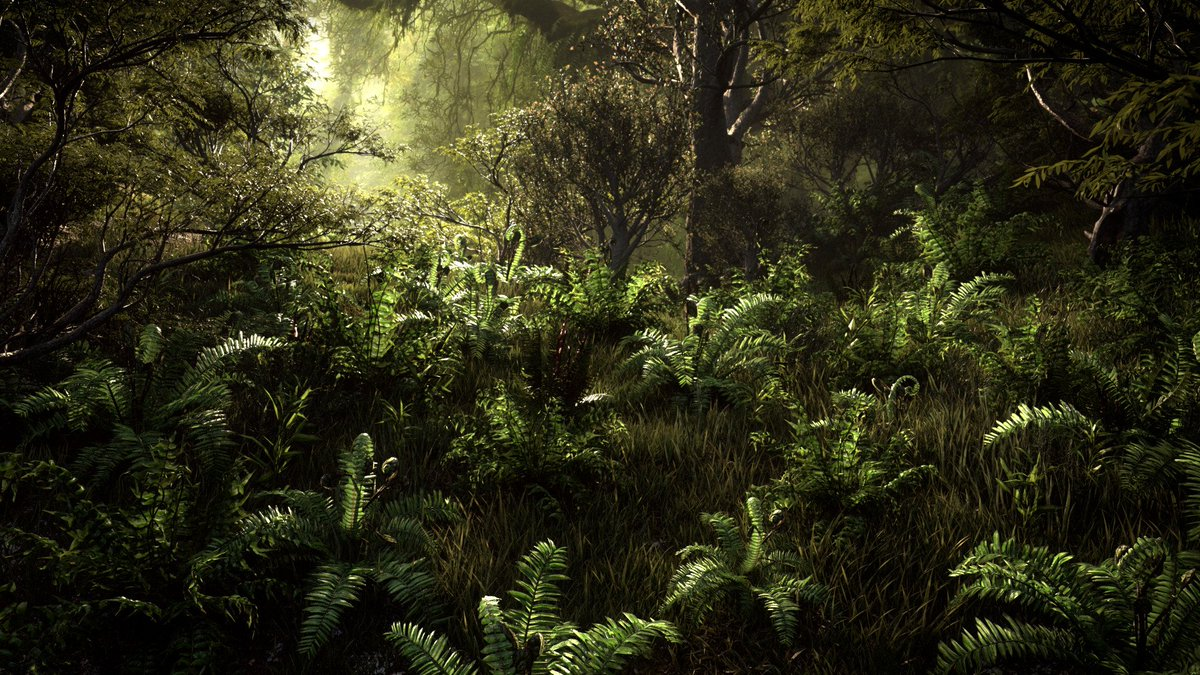
\includegraphics[width=0.8\linewidth]{Images/images/SpeedTree.jpg}
\caption{An example of environment filled with vegetation generated using \textit{SpeedTree}}
\end{figure}

Second, PCG can be used to increase replayability of games by creating new contents, missions, etc. For example, \textit{The Binding of Isaac: Rebirth}\footnote{Nicalis, 2013.} changes map layout and collectibles every match, therefore giving the ability to play a completely different match every time.

Lastly, PCG is so flexible that the whole concept of the game can revolve around it. The prime example of this is No Man’s Sky\footnote{Hello Games, 2016}, an exploration game where the whole world is generated with PCB, resulting in more than 18 quintillions\footnote{Specifically, 18.446.744.073.709.551.616 planets}  planets to explore, each with its own flora and fauna. Another great example is the Borderlands\footnote{Gearbox Software} series, where weapons are generated randomly by piecing together different parts, resulting, in the case of the first game, in more than 17,750,000 unique weapons.

\subsection{Procedural content generation with search algorithms}
PCG has attracted more and more academic interest in the years and many researches have been conducted to try and push PCG even further. While currently PCG techniques are rather simple and limited in scope, researches have been conducted to try to devise more elaborate generation algorithms and procedures to create more interesting content. This increased complexity however leads to a new challenge: evaluating the quality of the what is generated. 

The simplest approach, called \textbf{constructive PCG}, consists of, after generating content which passes some simple verification tests, letting a human decide whether the generated content is suitable for its purpose. 

%TODO Lanzi non aveva mostrato un sistema di generazione di tracce per un gioco di corsa dove all’utente venivano mostrate 8 mappe diverse e poteva scegliere la sua preferita, dettando così l’evoluzione? Potrebbe essere un esempio da mettere qui.

The problem of constructive PCG is that, by having a human in the equation, the entire process slows down and it’s impossible to exploit the full speed and generation capabilities of computers. For this reason the academic world is investigating a different approach for PCG, based around search algorithms and named \textbf{generation-and-test} or \textit{optimization-based PCG}, which attempts to automate the evaluation of the content to remove humans from the equation until possibly the very end of the process.

\textit{Generation-and-test} PCG is based around the fundamental concept of \textbf{fitness function}: a procedure used to evaluate how good a given content is for the purpose desired by assigning a real value or vector of real value representing its fitness. How the fitness function evaluates the quality of the content is an ad-hoc problem discussed in \Cref{section:fitness_function}. The fitness value assigned to each item is used to guide the generation process: individuals with higher scores have more influence over the generation of new ones. In this way, with time new contents will tend to have higher fitness values.

Using the fitness values to improve upon previously generated contents requires using a search algorithm, which allows us to scan a portion of the search space, representing the entirety of contents which can be created by the PCG procedure, in an attempt to find the highest valued content. 
The search algorithms used are often part of the larger family of \textbf{Evolutionary Algorithms} (EA): procedures which emulate natural biological evolution schemes, such as reproduction and mutation, to explore the research space.

When combining PCG and EA, the resulting procedure starts from an initial set of candidates, called \textit{population}, usually selected randomly and representing in some way the content to be evolved. 

Evolution happens in cycles, called epochs. Each epoch starts by a evaluating the \textit{fitness function} for each individual currently in the population. The fitness values computed are then used by the algorithm to choose which elements should be discarded and which ones should be preserved in the next epoch in a process called selection. After the selection, the surviving individuals can be kept as is, bred with others by employing cross-over or changed by using mutation in order to generate totally new individuals. The population obtained at the end represents the next generation and is the starting point for the process in the for the next epoch.

This process can be executed again and again, slowly exploring the search space until some stopping conditions, such as reaching the maximum number of epoch, finding a individual with a particularly high fitness value or loosing too much variance in the population, are met.

For a more detailed description of EA, interested readers can consult \cite{essentials_of_metaheuristics} and \cite{ea_critical_review}.

EA cannot usually work directly with the final content representation, be it a map, 3D model or anything else, it instead needs to use some encoded representation of the item. For this reason, in EA two concepts, again taken from biology, are introduced:
\begin{itemize}
\item \textbf{Genotype}: The low-level representation of the individual, the genotype encodes the individual as a set of parameters and values (e.g. string of bits, set of numbers) and is used by the evolution algorithm cross-over and mutation processes.
\item \textbf{Phenotype} The high-level representation of the individual, the phenotype is the actual content that is going to be generated and it’s the final product on which the fitness function is evaluated.
\end{itemize}

These two representation aren’t disjointed: there must be a way to map a genotype to the related phenotype in order for the evolution algorithm to work. Choosing a good genotype representation for the map and a valid mapping function from genotype to phenotype are two crucially important steps in preparing an EA,
since from those depends how efficiently the algorithm can explore the research space \cite{sbpcg_taxonomy}.

Using a genotype with too many parameters expands the search space, making it more likely to contain the optimal content to generate but causing the algorithm to converge to optimal solutions very slowly; on the contrary, too little parameters allow fast conversion but removes many potentially good elements from the search space. Finding a good balance is a complex problem named \textit{curse of dimensionality}\footnote{\url{https://en.wikipedia.org/wiki/Curse_of_dimensionality}}.

\subsection{Fitness function}
\label{section:fitness_function}
Using EA with PCG requires defining some key parts of the search algorithm, like the \textit{selection}, \textit{cross-over} and \textit{mutation} operators and the fitness function. Among those, the first three are usually relatively easy to define since many different techniques have already been studied and can be recycled for the problem at hand.

Defining a \textit{fitness function} instead is a complex, domain specific problem for which ad-hoc solutions must be devised. The main challenge to tackle is finding a clear correlation between parameters that can be measured by the function and what the user is trying to achieve by employing the EA; for example, measuring how strong or weak a specific generated weapon is is fairly easy; measuring how much enjoyment a human player might get from playing a generated map is hard, if not impossible. 

In fact, finding the right way to map what a human might think of a specific content is the main challenge of SB-PCG but it’s necessary to find a way to do so since, as stated before, bypassing the problem by letting the humans themselves judge the content (constructive approach) slows down the evolution process, making it impossible to explore the search space quickly and efficiently.

Fitness functions can be classified based on how they compute the evaluation metrics \cite{sbpcg_taxonomy}, and in particular we can identify:

\begin{itemize}
\item \textbf{Direct fitness functions}: The generated content is scored directly based on parameters of the phenotype. As an example, computing the average visibility of tiles in a map is a direct fitness function.
\item \textbf{Simulation-based fitness function}: The generated content is scored by extracting metrics out of simulations run using it. As an example, simulating matches on a generated map can be a great way to determine some of its characteristics, such as balance, which play styles it favours (e.g. close-range combat vs long-range combat), etc. They are extremely useful when it’s not clear how to evaluate the quality of the content by looking at its characteristics alone, but at the same time introducing this simulation step slows down significantly the evolution and introduces the problem of finding ways to realistically replicate interactions with the generated content. 
\item \textbf{Interactive fitness function}: The generated content is scored by gathering feedback from human testers. This approach allows to get realistic feedback on the content generated but is usually discouraged given that involving human actors slows down the process. Usually, it’s best to use this as a final step to validate the results obtained by the evolution.
\end{itemize}

\subsection{Procedural content generation for First-person shooters}
PCG of maps for FPS has been the focus of many studies in the years. One of the first works in this sense comes from Cardamone et al \cite{cardamone_evolving_maps} which tried to understand which kinds of map generated more interesting gameplay. To do so, the authors generated, using EA, maps for Cube 2: Sauerbraten\footnote{Wouter van Oortmerssen, Lee Salzman, Mike Dysart, 2004} based on four different structural representations and, by simulating matches on them, extracting the average time per fight, defined as the duration of the time range starting from the moment a player starts combat with another until the moment one of the two dies or escapes. The idea behind this choice is that, the longer this period, the more possibilities the map offers to escape, take cover, recover health and, in general, enact tactical strategies that make the game more interesting.

This research lead to two interesting results: first, its actually possible to use EA to evolve playable maps and second, the map representation had noticeable effect on the final results, so that some genotypes were better suited for the objective.

Starting from these results, Stucchi \cite{stucchi_evoluzione} tried to use EA to generate balanced maps for one-vs-one matches starting from any combination of players skills and equipment, using entropy as a kill ratio entropy as a the fitness function. The results showed how maps evolved to adapt their structure to bring advantage to the disadvantaged/less skilled player.

Arnaboldi \cite{arnaboldi_framework}, starting from Stucchi's result and setup, increased the quality of the simulations by improving the AI of Cube 2 bots used to run the games. This demonstrated one intrinsic problem of simulation based fitness functions: the quality of the result depends on the quality of the actors running the simulations; in order to get realistic results, the bots should behave as close as possible to a human agent.

Another problem in Cardamone et al’s approach was raised by Ølsted et al \cite{olsted_interactive_evolution_competitive} who noted how their system generates maps unsuitable for team-based multiplayer FPS like Counter-Strike, where the game focus develops around specific objective placed across the map. The same authors also note how the maps do not respect so called “rules of good combat”, such as guaranteeing multiple alternative paths, and therefore propose a new map generation and evolution approach consisting of randomly selecting nodes on a grid and evolving corridors, rooms, pickups and respawns connecting them to optimize such rules. 
This approach, based on the analysis of some \textit{Counter Strike} and \textit{Call of Duty} maps, further differentiates from Cardamone, Stucchi and Arnaboldi researches by using an interactive fitness function, since bot behavior was not deemed sufficiently human-like. Some criticism on their method can be raised however, considering that users involved in the map evaluation provided a simple binary answer concerning their appreciation of the map, without analyzing in more detail gameplay results or map characteristics 

Yet another approach to solve the map generation problem was tested by Bhojan Anand and Wong Hong Wei in \cite{bhojan_hong_arena}, which leveraged PCG with search based algorithms to quickly generate maps for Capture and Hold\footnote{Game mode first appeared in Killzone 2 and 3 (Guerrilla Games, 2009, 2011) in which two teams compete for the control of some strategic points. Team score increases periodically based on the number of controlled points; the team with the most points at the end wins} in an online fashion. By interconnecting pre-existing tiles representing open, zones and inaccessible zones, maps are scanned to detect regions which are then connected and filled with respawn points, flags and cover points. As fitness function, the authors opted for a direct approach, by computing metrics based on connectivity of region, collision points, flag position balance, in this way the evolution can be extremely fast and maps could be computed in a matter of seconds. However, the quality of the results, due to lack of simulation, can be contested and for this reason the obtained maps where later tested by human players which provided positive feedbacks.

\section{Balancing difficulty in video games}
In designing and developing a video game, extra care should be taken to ensure that the game experience is coherent with the concept desired. In particular, given a set of elements and mechanics a game is based on, a game is balanced if there exist no dynamic that, due to flexibility, strength or any other factor, outshines all the others. 

In an imbalanced game, some of the game features are ignored in favor of the stronger ones, leading to an impoverishment of gameplay and a waste of design and development resources, since weaker mechanics are ignored.

When discussing balance of game elements and mechanics, two terms are often used: \textbf{overpowered}, when something is much stronger than the rest, even after accounting for any possible cost for its usage, and, on the contrary, \textbf{underpowered}, when something is too weak even at the lowest cost of usage \cite{game_balance_concepts}.

Balancing game has two very different objective depending on whether the game is single or multiplayer.
 
In single player, balancing consists of ensuring that the level of difficulty of the game is adequate given the intended target. For example, the Dark Souls\footnote{From Software} series is known for its unforgiving nature and therefore it is expected that their difficulty is much higher than the standard for games of that genre.

In multi player, balancing consists of ensuring that no player has any intrinsic advantage over the others and no game strategy dominates the other in all or almost all situations. For example, in the fighting game Super Smash Bros. Brawl\footnote{Sora Ltd., 2008}, \textit{Meta Knight}, one of the playable fighters, had to be banned from competitive play because he was excessively overpowered and the whole metagame\footnote{The metagame refers to the collective decisions that are made outside of a game that affect tournament play. A metagame is said to have a "shape" or "state" which refers to the commonly employed practices and strategies in tournaments} was forcibly evolving around finding ways to counter it.

\subsection{Balancing of multi-player games}
Given the focus on this thesis, we will now focus on balancing multiplayer games.

As stated above, the presence of \textit{overpowered} or \textit{underpowered} elements in a game tends to cause a shift in gameplay mechanics since players who discover this imbalance will start taking advantage to it, forgoing usage of the weaker alternatives. With time, more and more player will then start using this unbalanced element and switch to dominant strategies revolving around this element, making the game more and more one-dimensional and, ultimately, boring, given the lack of variety.

While ideally a game should not have any overpowered element (and this can be mostly achieved only during design phase), it’s also a valid alternative to have more than one overpowered element, in order to let players choose the mechanic to “abuse” while still ensuring a basic level of variety.
%TODO Add more?

\subsection{Balancing of maps in video games}
In first person shooter and real-time strategy games, one of the most important elements to balance are the maps on which the game takes place. Designing balanced maps is a complex process for which no standard exist yet. The general approach followed starts from a designer pitching a possible draft for the map. The map proposed is then tested by human players in order to gather feedback from them and extract gameplay data (such visited positions, death positions, etc.), both of which are used to improve the initial design and try again with a new pitch, in a manner similar to EA cyclical evolution.

The main problem of this process is devising the first ever idea for the map: a badly designed map will require many iterations to get a final, working result. Due to this, many studies have been conducted to understand at least what properties make it a good multiplayer map \cite{pascal_multiplayer}, \cite{epic_multiplayer}, \cite{dodger_multiplayer}, \cite{larsenleveldesignpatterns} in order to leverage them during the design phase. 

Burgun \cite{keith_multiplayer} in particular focused on balancing, arriving at the conclusion that even perfectly symmetric maps might not ensure balance because their structure might nonetheless advantage some some weapons or strategies. 

Despite all the research on map properties and a plethora of studies on balancing maps for RTS games, very few have studies balancing for FPS.

\section{Summary}
In this chapter we analysed the current state of level design for videogames, identifying the reason behind our and other similar researches on the topic.
We then looked at \textit{Procedural Content Generation} techniques used in the years to support game development or entirely replace some tedious works. We focused on PCG using search algorithms, describing how they work and how they can be applied to support generation of maps for First-Person shooters.
Finally, we looked at the concept of difficulty in video games and what it means to balance difficulty in different contexts.



\chapter{Video game bots}
In this chapter we introduce video game bots by first describing what they are, what is their purpose and what can be considered a good bot.

We then proceed to analyze the general structure of a bot in order to understand how it gathers information from the world, how it decides what to do and how it interacts with the world to achieve its goals.

\section{What is a video game bot}
In video games, a bot is a type of artificial intelligence (AI)–based expert system software that plays a video game in the place of a human. 

Depending on the type of game being played, bots have very different purpose and structure. In particular, in multiplayer oriented FPS, a bot is an artificial player whose purpose is to replace a human to serve either as a teammate or an enemy to the real player(s). Such types of bots are subjected to the same (game) rules that apply to human players but interact with the game in a very different way. While a human player uses classical input/output interfaces, like mouse, keyboard, computer monitor and the likes, a bot interacts directly with the game by receiving information about the virtual world (as a set of variables) and using the knowledge gained through them and provided in advance to calculate and send sequences of commands to respond to the evolution of the virtual world. In order to ensure fairness, it's important that these actions are very similar to the actions a human player can input using the computer’s input devices.

\section{Perfect bot vs enjoyable bot}
What is a \textit{good} bot?  In order to answer this simple question we must first ask ourselves: what are we trying to achieve by creating such bot?

Depending on the field, bots can have very different purposes. \\
As an example, consider chess. Numerous artificial intelligence researches and studies have been conducted on the game of chess in order to try to create the perfect bot, one that combines superhuman prediction and analysis capabilities to always chooses the optimal move, making it difficult or impossible for humans to checkmate the AI.

In a FPS game, playing against a bot which is always choosing the optimal action every time would quickly get boring or frustrating, since a human player would have little to no chances of winning. From this simple consideration, it should be clear that the purpose of bots in FPS is not to play optimally, but rather try to play exactly as a human player would, so a good bot here would be one that virtually cannot be distinguished from a real player \cite{fun_human_bots}.

Simulating the behavior of a human is of course not an easy task, although thanks to the increase in processing power some promising results have been achieved, for example in \cite{ai_reinforcement_learning}. 
%TODO reprase here % 
It should be noted however that, since this kinds of researches use techniques such as reinforcement learning which generate very complex mathematical models, it is still not possible to know exactly how the bots achieve human like behavior. Moreover, reinforcement learning requires training by analysis of real matches, and the amount of data required means that its impossible to successfully train such bots before a game is released, so for now human-like bots are not being investigated by the industry and remain instead a niche research of the academical world.

\section{Structure of a video game bot} \label{section:bot_theory}
While there are countless ways to design and implement AI for video games, at a theoretical level it is possible to identify three key conceptual areas they all have in common:
\begin{itemize}
\item \textbf{Knowledge acquisition and processing}: involves processing data and information that has been programmed directly into the bot or acquired during gameplay.
\item \textbf{Decision making}: takes care of making all decisions about the actions that a bot takes.
\item \textbf{Actuation}: involves all the components which allow the bot to interact with the game world.
\end{itemize}

For the remainder of the chapter we will analyze these 3 topics.

\subsection{Knowledge acquisition and processing}
In order for a bot to make informed decisions about how to act, it must first understand the game world: its composition, the criteria for its evolution, and the rules of the game. It also needs to be able to observe the state of the world to react appropriately to changes.

These aspects can be broken down into three fundamental components that make up a bot's knowledge:
\begin{itemize}
\item \textit{Domain knowledge}: The set of rules that define how the game works and how the state of the world changes over time.
\item \textit{Cognitive model}: The collection of data and information that encode the state of the game world.
\item \textit{Knowledge acquisition}: The techniques the bot uses to observe changes in the game world and potentially learn new emerging dynamics.
\end{itemize}

\subsubsection{Domain knowledge}
In order to be able to play, a bot needs to know the general rules of the game, the environment and their evolution. This knowledge is referred to as \textit{domain knowledge} and is required to allow the bot to reason about the effect of its actions to reach its goals. 

Basic \textit{domain knowledge} includes rules about:
\begin{itemize}
\item How the state of the world changes upon user interaction: for example, walking in the same space of a medkit will remove it from the game and heal the user; interacting with a specific button activates or deactivates an elevator nearby, etc.
\item How the state of the world changes by itself with the passage of time: for example, a collected medkit will respawn after some time has passed; an activated elevator moves up or down, etc.
\end{itemize}

More advanced domain knowledge might also contain strategic information that helps the bot reason about its behavior and the behavior of others. Looking a enemy fleeing a fight, for example, might suggest the bot to go patrol an active medkit nearby to ambush the opponent. This kind of knowledge is the most complex to represent and use.

\subsubsection{Cognitive model}
After having learned the basic rules to play a game, players encountering a new environment have to learn how to play in it. To do so, humans have to explore the map and, starting from the rendered virtual world, create their own internal representation of the environment. This simplified representation will help them navigate, find cover points, choke points, etc., without the need to remember all the details of the original visual representation.

In a similar fashion, a bot must be provided with a cognitive model of the map in order to perceive and understand the virtual world. This cognitive model must be comprehensive, since any aspect of the world not represented within it cannot be perceived by the bot, but also efficient, meaning that accessing and reasoning about the world must be quick enough. Achieving both these contrasting characteristics it's possible by cutting away many unnecessary information (like colors and textures), pre-baking useful information (like waypoints to facilitate navigation) and adding any additional metadata that can better describe a specific location (e.g. cover point), object (e.g. medkit that heals 80 points), or entity (e.g. their team).

\subsubsection{Knowledge acquisition}
An effective bot must be able to detect the evolution of the world state to properly play a match. This knowledge acquisition is known as \textbf{sensing}. 

While a human player would have to interpret the state of the world though the output devices of the computer, a bot will receive this information directly through the game as a set of variables.

This opens up a problem: while a human can acquire only information about things that it can directly see or hear, a bot can potentially access the whole world state, including information that shouldn't be accessible all the time, like enemy positions. A good bot should refrain from cheating, although cheating can be used sometimes as a shortcut to give the agent some semblance of intelligence. As an example, skilled players might be able to correctly predict the location of enemies which recently respawned and a bot can achieve the same by directly accessing the real position (or a slightly skewed one). 

Given that the knowledge a human player gains is limited by what it hears or sees, a bot should try to limit the amount of data acquired based on those senses. For example, a player can only see things that are displayed on the monitor because they fall in the camera field of view, and in a similar fashion a bot should be able to see only things that are in front of him. Other factors, such as fog, foliage, shadows and such might limit visibility and a properly implemented bot should take those into account as well. Similar considerations hold for audio, for example humans struggle to understand from where a specific sound comes from when multiple sources are present, in the same way a bot, when exposed to different noises, shouldn't be able to automatically pinpoint the location of each source.

Aside from world state knowledge, the bot might also try to understand world dynamics emerging during gameplay, such as enemy patterns in movement. This kind of knowledge acquisition, called \textbf{learning}, is much more complex than \textit{sensing}, as it requires the recognition of patterns in a large of series of observation and evaluation of the effects of certain sequences of actions. Advanced techniques such as neural networks can be used to achieve \textit{learning}. 

\subsection{Decision making} \label{subsection:theory_decision_making}
Besides having and gaining knowledge, the bot must act by deciding on its own what to do based on what it knows and has to accomplish.
Bot behavior is determined by the choice of the goal it wants to achieve and the sequence of action needed to achieve that goal. 
Both the choice of the objective and the action plan can be static, making the bot very predictable, or change dynamically and/or randomly, making the bot unpredictable and more similar to a human player.
There are three extremely popular ways to code the bot behavior, \textit{Finite State Machines}, \textit{Goal-Oriented Action Planning} systems, and \textit{Behavior Trees}.

\subsubsection{Finite state machines}

A finite state machine (FSM) is a mathematical model of computation representing a system that can be in exactly one of a finite number of states at any given time. The FSM can change from one state to another in response to some inputs; the change from one state to another is called a transition. Using a FSM to represent a bot behavior means encoding its states and the transitions between them and mapping the various states to an action or sequence of actions to perform.

The graphical representation of an FSM is easy create and understand, since there are only two concepts, states and transitions, to model. An example of FSM for a bot is shown in \Cref{fig:fsm_bot}
%, representing the behavior of a generic bot in a first person shooter like Doom. This bot can, at any moment, be in 4 different states, gathering items, retreating from a fight, attacking an enemy or chasing an enemy. For what concerns transitions, an attaching bot can transition to any other state, a bot gathering items can only start attacking and bot who are retreating or chasing  can either start attacking or move on to gather items.

FSM are very easy to implement but tend to be complex to maintain, since for every new state added many different transitions and their conditions must also be included, up to the point where adding anything new is prohibitively difficult.
%TODO add citation for something (e.g. for HFSM)
Due to this, different evolutions of FSM have been proposed in the years, for example, Hierarchical Finite State Machine use different, nested FSM to better decompose the various states and reduce the amount of states and transitions in each layer.

\subsubsection{Goal-oriented action planning systems}
Goal-Oriented Action Planning (GOAP), refers to a simplified STRIPS-like planning architecture specifically designed for real-time control of autonomous character behavior in games. GOAP was initially implemented to model the AI for F.E.A.R. and later inspired many research on the topic. In GOAP, a bot has a collections of possible goals it wants to achieve and a representation of the steps required to reach them. Steps can be elementary actions or (sub)goal themselves; this goal nesting capability allows building complicated action plans with ease.

\subsubsection{Behavior trees}
\textbf{Behavior Trees} (\textbf{BT}) are a formal, graphical modelling language used primarily in systems and software engineering. A BT models an execution plan for a specific task using a graphical representation based on an directed acyclic graph. An example of BT is shown in \Cref{fig:tutorial_bt}

Behavior trees became popular for their development paradigm: being able to create a complex behavior by only programming the NPC's actions and then designing a tree structure (usually through drag and drop) whose leaf nodes are actions and whose inner nodes determine the NPC's decision making. Behavior trees are visually intuitive and easy to design, test, and debug, and provide more modularity, scalability, and reusability than other behavior creation methods. 

It should be noted that, due to their simplicity and versatility, BT have been often abused to represent more than just action plans, as noted by Anguelov \citep{bt_abuse}, so often BTs are even used to control the state of the bot, leading to complex to maintain and poorly scalable AIs.
\begin{figure}
\begin{center}

\includegraphics[width=0.4\linewidth]{Images/images/FSM.drawio.png}
\caption{Example of Finite State Machine for a generic bot in an FPS game}
\label{fig:fsm_bot}
\end{center}
\end{figure}
\vspace{1cm}
\begin{figure}
\begin{center}
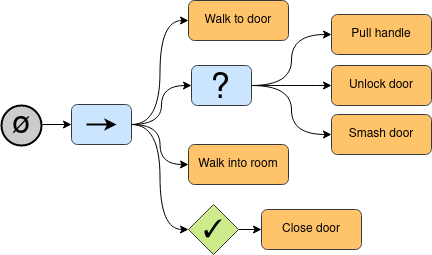
\includegraphics[width=0.5\linewidth]{Images/images/BTTutorial.drawio.png}
\caption{Example of a Behavior tree for the task of entering a closed room.}
\label{fig:tutorial_bt}
\end{center}
\end{figure}
\vspace{1cm}
\begin{figure}
\begin{center}
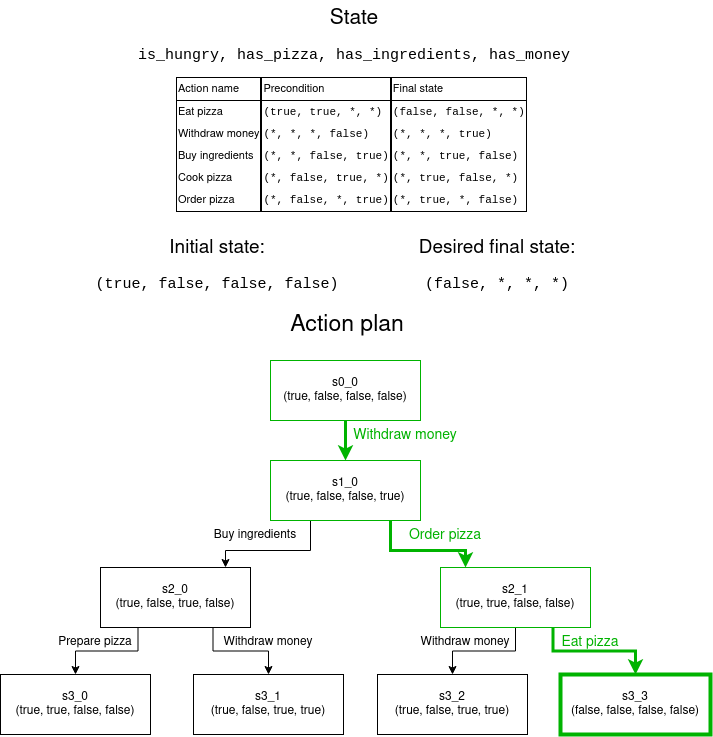
\includegraphics[width=0.8\linewidth]{Images/images/GOAP_NEW.png}
\caption{Example of GOAP to prepare dinner.}
\label{fig:tutorial_goap}
\end{center}
\end{figure}

\subsection{Actuation}
After having chosen the course of action to follow, a bot must take those actions. In order to do so, the bot has to interact with the game engine in order to walk, jump, shoot, reload, and so on.

The actions that a bot can take should subjected to the same limitations a human player has, both accounting for the game rules (e.g. a bot should not move faster than a normal player) and the real world rules (e.g. a bot should not be able to instantly turn around and aim towards an enemy given that this action executed with a mouse would take some time to complete).

\section{Summary}
In this chapter we analysed the high-level architecture of a video game bot, in order to better understand the AI we developed in this research to support our purposes. 
We also briefly discussed some of the nuances of creating a perfect bots versus an enjoyable one in order to understand when either one is more suited.



\chapter{Unity framework}
The purpose of this chapter is to describe the Unity framework used to automate game testing. 
The framework used is an extension of initially developed by Ballabio \cite{ballabio_framework} capable of running automated 1 vs 1 matches on dynamically loaded maps between bots with configurable parameters.

\section{Motivation for the framework}
%TODO
Academic research on map generation for FPS is still newborn and there isn't yet a consensus on the tools to use. Most researches followed the example from Cardamone and used Cube 2: Sauerbraten as their starting engine, later customized to fit the needs of the research. Others, for example Bhojan Anand and Wong Hong Wei in \cite{bhojan_hong_arena}, opted to create their own game engine, a complex tasks which doesn't really pay off if used for a single research.

Given that game development has evolved in the years and it's now easier to code games using more modern tools and engines, for example Unity\footnote{https://unity.com/} or Godot\footnote{https://godotengine.org/}, it should be now feasible to produce a new, rather generic framework that can be easily customized to adapt it to any possible research one wants to conduct.

For this reason in his thesis Ballabio \citep{ballabio_framework} developed a new Unity framework which offers a plethora of useful capabilities for any kind of experiment, most notably the possibility of building and embedding the game in a web page, allowing researches to gather data from users playing from anywhere in the world, without requiring any complex installation or setup on their machines.

However, Ballabio's framework had a big shortcoming in the lack of bots, an essential tool to run any kind of simulation required by many techniques, such as Search Based Procedural Content Generation. Bots have been introduced with our work in this thesis and will be described in \Cref{section:unity_bots}.

\section{High-level overview}
In order to help readers follow through the explanation of our study, a small overview of Ballabio’s framework main concepts is given below. For more details readers are advised to consult \cite{ballabio_framework}.

\subsection{Map representation}
Maps are structured as grids of orthogonal tiles and are internally represented by matrices of characters, where each cell corresponds to a specific tile. Each tile can represent either an empty space, a wall, an ammo pack, a medkit, a spawn point or stairs. 
In case the map has multiple floors, each floor is represented by one such matrix of characters. An example of map can be seen in \Cref{fig:char_map}.
Independently from how a map is initially represented (e.g. all-black, cellular, …), it must always be converted to this format.

\begin{figure}[hbtp]
\centering
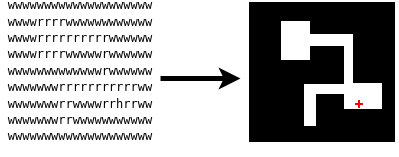
\includegraphics[width=0.7\linewidth]{Images/images/charmap.drawio.png}
\caption{Mapping of matrix representation of the actual map. The black areas are non-walkable spaces, the '\textcolor{red}{\textbf{+}}' is a medkit.}
\label{fig:char_map}
\end{figure}


\subsection{Game manager}
The \textbf{Game Manager} is the module responsible for the overall behavior of a match. Different implementations of \textit{Game Manager} exist, each representing a different type of match and handling its entire life cycle, from setup to the final scoring.

\subsection{Map Manager}
The \textbf{Map Manager} controls the generation or the import and the assembly of the map and the displacement of objects inside it.

For the generation of the maps and displacement of spawn points and pickups it uses the \textit{Map Generator}, of which various versions exist depending on the specific generation algorithm (e.g. digger), while for the conversion from text representation to the final 3D map the \textit{Map Assembler} is employed.

\subsection{Experiment manager}
The \textbf{Experiment Manager} is a stand alone module that allows to create and manage the experiments used to perform user-based validation. Once an experiment has been defined, the \textit{Experiment Manager} automatically assigns to the users the matches to play and collects the desired information.
Given that our research doesn’t involve any interaction with the user, we didn’t use any \textit{Experiment Manager} in our project.

\subsubsection{Entities}
The \textbf{entities} are the agents that take part in a match.
In their most basic form, an \textit{entity} essential parameters are its position, health and weapons. Given that one of the focus of our project was implementing an AI in the game, entities will be described more in \Cref{section:unity_bots}.

\subsubsection{Weapons}
Any kind of firearm used by entities, defined by parameters such as their type (raycast, projectile, laser), damage, projectiles per shot, reload time, …

\subsubsection{Game modes}
Ballabio’s framework supports 3 different kinds of mode, \textit{Duel}, \textit{Target Hunt}, \textit{Target Rush}. For the purpose of our research, we focused only on \textit{Duel}, which represents a simple 1-vs-1 deathmatch with respawn.

\section{Data gathering and processing}
To perform any kind of experiment, we need to be able to gather data from various matches for further processing. 

Our framework is capable of saving a lot or raw data coming from matches. This data is then analysed outside of Unity to extract some interesting metrics. In the following sections we will describe the data gathered and how it is processed.

\subsection{Match raw data}

For every match, the framework gathers the following data, which measures characteristics determined by the map topology:

\begin{itemize}
\item \textit{Time to engage}: Measures the time between the end of a combat event and the next one, or, right at the beginning of the match, between the respawn time and the first combat start.
\item \textit{Time in fight}: Measure the total time a bot spends fighting an enemy, considering also the time spent searching it right after losing its tracks.
\item \textit{Number of fights}: Total number of fights.
\item \textit{Time between sights}: Total time between the moment an entity can no longer detect an enemy and the moment it is detected again, considered for every fight event.
\item \textit{Number of sights}: Number of time an enemy return sighted after becoming undetected.
\item \textit{Time to surrender}: Time between the moment a bot loses track of the enemy and the moment it decides to abort searching for it.
\item \textit{Number of retreats}: Number of times a bot abandons searching an enemy after a fight.
\end{itemize}

Additionally, for each entity in the game, the following data is measured:

\begin{itemize}
\item \textit{Frags}: Number of kills performed by the entity
\item \textit{Deaths}: Number of deaths of the entity.
\item \textit{Shots}: Number of bullets fired by the entity.
\item \textit{Hits}: Number of times a projectile shot by the entity hit an entity (including itself).
\end{itemize}

\subsection{Analysis metrics}
By taking inspiration from some of the factors that experts in the field identified as required for the creation of good maps (\cite{game_design_secret_sages, best_multiplayer_maps_one, best_multiplayer_maps_two}), we selected some metrics measuring interesting aspects during the design of levels.

\subsubsection{Balance}
Map balance, interpreted as the possibility offered by the map to achieve a fair match between participants, is possibly the most important characteristic to observe, especially for multiplayer games. While balancing could be obtained by simply using symmetrical maps (as done in \textit{Splatoon}\footnote{Nintendo, 2015}), a good, balanced map should offer a good balance between advantage and disadvantage situations in order to allow each side to contrast the others.
Weapons usually offer a significant tactical advantage versus others in some specific situations. Shotguns for example are better suited for short-range combat, while sniper rifles excel at long-range. Map structured in specific ways could therefore favour only a single type of game style. 
An effective way to measure the efficiency of a player is by computing the kill/death ratio: the best players are those that can kill others without attracting too much enemy fire.
To evaluate the balance we opted to use the \textbf{entropy} of all kills, used by both Stucchi \cite{stucchi_evoluzione} and Arnaboldi \cite{arnaboldi_framework} to generate balanced maps.

\begin{equation}
entropy = \sum_{i=1}^{n} - \left( \frac{k_i}{k_{tot}} \right) \log_2 \left( \frac{k_i}{k_{tot}} \right)  
\label{eq:entropy}
\end{equation}

In formula \eqref{eq:entropy} $k_i$ represents the number of frags of the i-th bot, while $k_{tot}$ is the total number of frags in a match.
Entropy values vary in the the [0-1] range: values close to zero indicate a wildly unbalanced match in which a player trumped all the others, while values close to 1 represent balanced matches.

\subsubsection{Pace}
Another important aspect of matches to keep track of is frequency of encounters between players. Matches which evolve too slowly, with very few battles between sides, would result boring and not particularly engaging. On the contrary, too high frequency encounters would make players feel overwhelmed and would prevent any sort of tactic, making the experience frustrating.
To compute a \textit{pace} value normalized in the [0,1] interval the following function \Cref{eq:pace} was used.

\begin{equation}
pace = 2 * \frac{1}{1 + exp \left( -5 * \frac{NumberOfFights}{\sum TimeToEngage} \right) } - 1
\label{eq:pace}
\end{equation}

The sigmoid function \Cref{eq:pace} computes values for \textit{pace} close to 0.9 for average time to engage equal to 3 seconds. %TODO verify number

%TODO add other metrics in case they are needed

\subsection{Performance metrics}
Besides metrics measuring characteristics of the map, it's useful to keep track of other metrics regarding the performance of the different bots during matches.
The metrics we extract are:
\begin{itemize}
\item \textbf{Number of Frags} Total number of frags in a match.
\item \textbf{Accuracy} How precise each bot is when shooting, calculated as the ratio between the number of \textit{Hits} and the number of \textit{Shots}.
%TODO missing metrics from Arnaboldi
\end{itemize}

%TODO not sure whether all the metrics above are ever used, so we can probably not describe them for the time being.


\section{Unity bots} \label{section:unity_bots}
In this section we'll be analyzing the bots we developed for our research. We will first be briefly discuss their architecture and later focus our attention on how they work by studying one of their processing cycles. 

\subsection{Bot architecture}
The AI of the bots we developed is structured as a modular system, composed of four distinct layers, each with its own specific responsibilities. This design, which can be seen in \Cref{fig:modular_layered_bot} allows for a clear division of responsibilities and ease of maintenance, as changes can be made to individual layers without affecting the entire system.

\begin{figure}
\centering
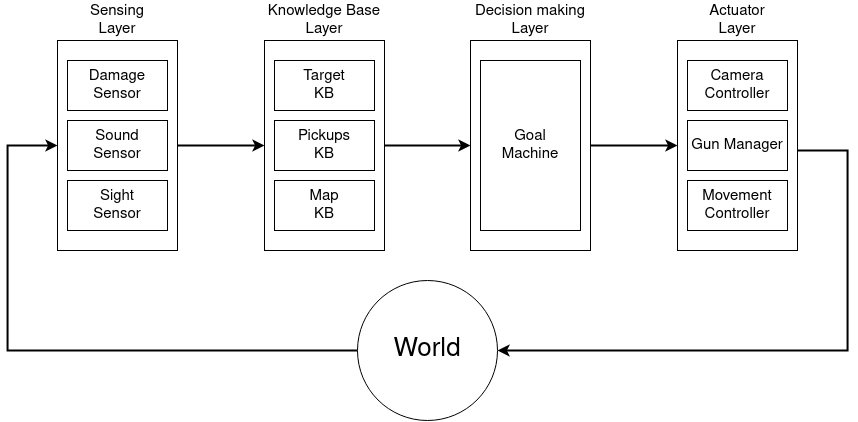
\includegraphics[width=0.8\linewidth]{Images/images/LayeredArchitecture.drawio.png}
\caption{Bot layered architecture and information flow between the layers and the world.}
\label{fig:modular_layered_bot}
\end{figure}

The \textbf{Sensing layer} is one of the two interfaces the bot has with the in-game world and it is in particular responsible  of receiving inputs from the environment in order to provide access to this information to the following layer. Examples of data sensed by this layer are sounds from guns firing, damage received by the bot and visual information such as the visibility of an item or entity.

The \textbf{Knowledge Base layer} is responsible for storing and processing all relevant information about the game world, both learned through \textit{sensing} and given as initial domain knowledge. This layer acts as a repository of information that the bot can use to make informed decisions. The information provided by the \textit{Knowledge Base} can include last known locations of enemies, the shortest paths to different destinations, the location, estimated activation time and effectiveness of different pickups and so on. By using this information, the bot can make informed decisions and execute effective strategies within the game.

The \textbf{Decision Making layer} is responsible for determining the objectives and action plans for the bot based on the (perceived) current state of the environment and the bot itself. This layer evaluates various options and chooses the one that is most likely to lead to success, given the information available from the \textit{Knowledge Base}. Examples of decisions made in this layer include whether to attack or flee from an enemy; whether to track a lost enemy or instead collect health or ammo supplies and so on. The \textit{Decision Making layer} continuously strives to maximize the bot chances of success by carefully weighing the potential outcomes of each available action.

Finally, the \textbf{Actuator layer} is responsible for executing the actions determined by the \textit{Decision Making layer}, translating them into actual in-game interactions such as moving around, rotating the view, shooting, reloading, and switching weapons, which ultimately allow the bot to interact with the virtual world.

A more in-depth description of how the different tasks of each layer are handled is provided in the following sections.

\subsection{Sensing layer}
The \textit{Sensing layer} purpose is to receive raw data from the world in order to allow other layers to process it.
It important to notice that this layer only checks if an event happens, other layers are then responsible to understand if the bot should react to such event. This means, for example, that an enemy being visible according to the \textit{Sight sensor} doesn’t necessarily mean that the bot can/should immediately react to it; rather, upper layers will usually introduce some delay to simulate reaction time of a normal human.

The \textit{Sensing layer} is composed of three different modules.

\subsubsection{Sight sensor}
Takes care of determining whether a given location, item or entity is currently visible by the bot, based on three criteria:
\begin{description}
\item[Presence of obstacles] If an obstacle, such as a wall, ceiling or other entity fully covers the target, then it won't be considered visible. In order to check this, the Unity raycast function is employed.
\item[Bot field of view] If the target is outside the cone of vision of the bot, then it's not visible;
\item[Bot depth of view] If the target is too far away, the bot won't be able to see it.
\end{description} 
%TODO image about sight, hear

\subsubsection{Sound sensor}
The \textit{Sound Sensor} is responsible for detecting and determining the origin of sounds in the game world. Currently, the only source of noise in the game is gun fire, whose volume depends on the type of weapon fired. Then, depending on the distance of the sound source and the sensitivity of the bot, the bot might detect or not that a shot was fired.
%TODO image about sight, hear


\subsubsection{Damage sensor}
Finally, the \textit{Damage sensor} takes care of detecting whether an entity received damage recently.


\subsection{Knowledge Base layer}
The \textit{Knowledge Base layer} purpose is analyzing data received from the \textit{sensing layer} and, combined with knowledge of the world provided in advance, provide tactical information to be used by the \textit{Decision layer}.
There are three modules in this layer.

\subsubsection{Target knowledge base}
\label{subsubsection:target_knowledge_base}
The \textit{Target Knowledge Base} module is responsible for determining the presence and position of enemies according to the bot. 
Before understanding exactly how this component works, it's crucial to understand the difference between a visible target and a detected target.
 
A visible target is one that is currently visible to the bot based on the information provided by the \textit{Sight Sensor}. 

A detected target, on the other hand, is one that has been visible for a sufficient amount of time that the bot can react to its presence and will continue to remain detected until after a while it is no longer visible. 

By allowing enemies to be visible, but not detected according to the knowledge base, it is possible to emulate reaction delays of a typical human player.

According to the \textit{Target Knowledge base}, a target can be in three different states:
\begin{description}
\item[Detected] The target recently remained visible for enough time for the bot to notice. The amount of time is inversely related to the distance of the target, so that the bot reacts faster the closer the enemy is\footnote{A more accurate analysis on reaction time and distance can be found in \cite{rabin_reaction_time}}.
\item[Lost] The target isn't currently detected, but was detected until recently.
\item[Undetected] The target isn't detected and wasn't considered detected recently.
\end{description}

Knowing whether an enemy is considered detected or not is crucial for upper layers to understand whether we know its exact location (when detected), can only approximate it (when lost) or if the whereabouts are unknown (when undetected).

\subsubsection{Pickup Knowledge Base}
%TODO

The \textit{Pickup Knowledge Base} keeps track of all the pickup items present in the map. Its main responsibilities are determining the location and effect of all pickups, as well as providing precise or estimated data about their past, present, and future status.

This last part is especially critical: since pickups become temporarily disabled after being collected, the knowledge base must be able to determine whether a bot can pickup something or not at any given time.

In order to do so, the \textit{Pickup Knowledge Base} internally keeps track of when the pickup was last seen, when it was last seen active and what is the latest estimated activation time. All this information is updated whenever a pickup is visible. 

Using this information to estimate activation times is pretty straightforward, in particular, if a visible pickup is currently active, then its status is obviously active, while in case it is disabled, the estimated activation time is computed as the current time plus half the normal pickup delay or the current estimated activation time, whichever is higher.

Additionally, if a bot recently collected a pickup, there is no need to estimate the next respawn time, it will be set to the normal pickup cool-down.

%TODO Maybe remove?
\subsubsection{Map knowledge base}
The \textit{Map Knowledge base} is used to keep track of when any specific area of the map was last visited. Keeping track of this information can help the bot decide what should be the next area to inspect or predict where an enemy might be located.

\subsubsection{Navigation system}
The \textit{Navigation system} is a critical component responsible of calculating the path of an agent to a given destination, keeping into account the topology of the map and any obstacle along the way. Without this component traversing the game map wouldn't be possible.

Currently, our \textit{Navigation system} relies on the Unity Navigation and path finding system\footnote{https://docs.unity3d.com/Manual/Navigation.html}.

\subsection{Decision making layer}
The \textbf{Decision Making layer} has the task of, given the current state of the bot and the environment, choose the objective that should be pursued and, as a consequence, the action plan to follow.

In order to obtain a rather flexible, yet easy to understand and maintain AI, we opted to mix together some of the decision making techniques discussed in \ref{subsection:theory_decision_making}, ultimately creating a fuzzy, state-based decision making system backed by action plans defined by behavior trees.

In our system, the bot has currently 4 possible states representing what the bot is currently trying to achieve: \textbf{Wander}, \textbf{Fight}, \textbf{Collect pickup} and \textbf{Search enemy}, which will be described in detail in the next sections.

No transition between these states is defined; rather, depending on the bot current status and knowledge, each state calculates a \textit{score} and at any time the state with the higher score is the current one. This system makes it possible for the bot to change its behavior as a response to any possible event without the need for the programmer to explicitly define this reaction, ultimately making it possible to add new states by simply defining their score function without having to worry about integrating this new state with the others.

Each state uses a behavior tree to define the sequence of actions that the bot will take to achieve the objective of the state itself. Using a graphical tool such as behavior trees makes it incredibly easy for everyone, even without programming knowledge, to visualize, modify and tweak the behavior of the bot in each of the states.

In order to simplify a little bit the visualization of the Behavior Trees, the various images presented in the next sections will separate between the action plan governing the momement of the bot and the action plan governing instead camera and guns.

For a detailed reference on the syntax used for Behaviour Trees, check \ref{section:unity_bots} in the Appendix.

\subsubsection{Wander}

\begin{figure}[hbtp]
\centering
\begin{subfigure}[c]{0.4\linewidth}
	\centering
	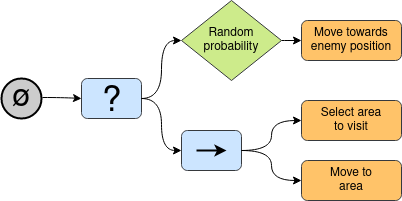
\includegraphics[width=\linewidth]{Images/images/WanderMovement.drawio.png} 
	\caption{Movement}
\end{subfigure}

\begin{subfigure}[c]{0.3\linewidth}
	\centering	
	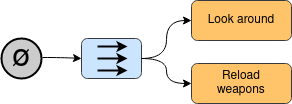
\includegraphics[width=\linewidth]{Images/images/WanderHead.drawio.png} 
	\caption{Camera and guns}
\end{subfigure}

\caption{Behaviour Trees governing the actions of the bot while wandering}
\label{fig:wander_bt}
\end{figure}

%
%\begin{figure}
%\centering
%\captionsetup[subfigure]{}
%\subfloat[\centering Movement]{
%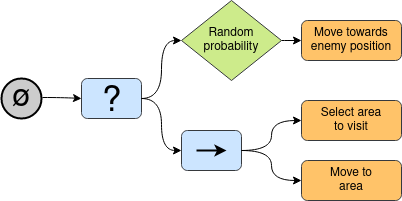
\includegraphics[width=0.3\linewidth]{Images/images/WanderMovement.drawio.png}} 
%
%\subfloat[\centering Camera and guns]{
%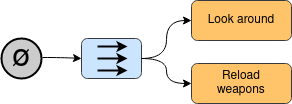
\includegraphics[width=0.4\linewidth]{Images/images/WanderHead.drawio.png}} 
%\caption{Behaviour Trees governing the actions of the bot while wandering}
%\label{fig:wander_bt}
%\end{figure}

When a bot is in \textit{Wander} state, pictured in \Cref{fig:wander_bt}, it has no specific objective, like collecting a pickup or chasing someone, and it will just roam around the map in the hope of stumbling upon the enemy. As such, this state tends to be a last resort and has therefore a very low score.

When wandering, a bot will constantly do three things in parallel:
\begin{itemize}
\item \textbf{Move around}: The bot will explore the map by selecting a random destination to reach, giving more preference to places not visited recently. In order to allow emulating skilled players, which might be able to estimate from the match progression where an enemy is, when selecting a destination there is a probability (settable by the user) to choose the enemy position.
%TODO Probability is not settable by user at the moment
\item \textbf{Look around}: The bot scans the area, hopefully finding enemies before they find it. 
\item \textbf{Reload weapon}: If the bot possesses any weapon not fully loaded, there is a chance it might start reloading them. The bot doesn’t just eagerly reload weapons in order to give some level of unpredictability.
\end{itemize}

\subsubsection{Collect pickup}
\begin{figure}
\centering
\captionsetup[subfigure]{}
\subfloat[\centering Movement]{
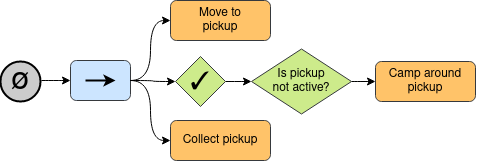
\includegraphics[scale=0.5]{Images/images/PickupMovement.drawio.png}} 

\subfloat[\centering Camera and guns]{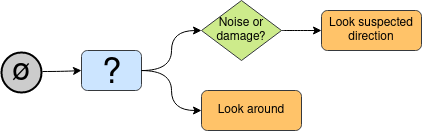
\includegraphics[scale=0.5]{Images/images/PickupHead.drawio.png}}
\caption{Behaviour Trees governing the actions of the bot collecting a pickup}
\label{fig:pickup_bt}
\end{figure}

When running low on health or ammo, a bot might decide to switch to the \textbf{Collect pickup state} (\Cref{fig:pickup_bt}) in order to collect the med-kits and ammo crates scattered through the map.

The score assigned to this state is computed as the maximum score assigned to all pickups in the map.

The bot calculates the score of each pickup based on the following factors:

\begin{itemize}
\item Absolute value of the pickup: Pickups that restore a higher amount of health or ammo are given higher scores.
\item Relative value of the pickup: The bot takes into consideration its current health and ammo levels and values pickups more highly the lower its current levels are.
\item Proximity to other pickups: Pickups located close together are given higher scores as they can be collected more efficiently.
\item Time to collect pickup: Pickups located closer to the bot's current position are considered safer and more valuable as they can be collected quicker.
\item Uncertainty of the pickup status: If the bot is uncertain about the availability of a pickup, it is considered a higher risk and given a lower score.
\end{itemize}

Once the pickup to collect is chosen, the bot will compute the shortest path to reach it and start moving towards it, while keeping an eye open for danger. This is achieved by looking around and turning immediately in case noise was heard or damage was received.
Once the correct location of the pickup is reached, the bot will remaining in the area, waiting for it to respawn if needed, and then proceed to collect it.

One important thing to notice is that the bot knowledge is continuously being updated, so at any time the score assigned to a pickup might change as a result of new information acquired and, consequently, the score assigned might change, potentially resulting in switching the pickup to collect.

As an example for this, imagine that the bot was headed to collect a pickup which believed to be active but, upon reaching its location, discovered it wasn’t. If another pickup is close by, the bot might decide to avoid waiting for the currently selected one to respawn and instead opt to fetch the other one.

\subsubsection{Search enemy}
\begin{figure}
\centering
\captionsetup[subfigure]{}
\subfloat[\centering Movement]{
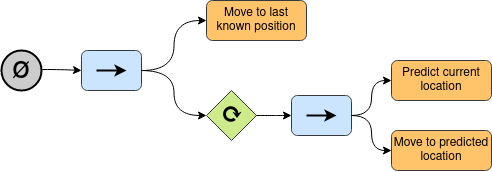
\includegraphics[scale=0.5]{Images/images/SearchMovement.drawio.png}} 

\subfloat[\centering Camera and guns]{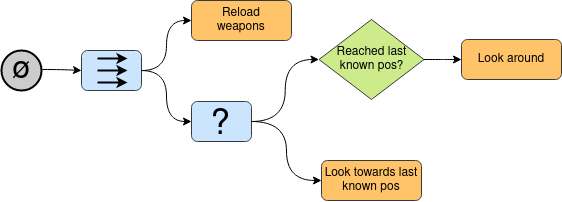
\includegraphics[scale=0.5]{Images/images/SearchHead.drawio.png}}
\caption{Behaviour Trees governing the actions of the bot searching an enemy}
\label{fig:search_bt}
\end{figure}

Any time the bot hears a suspicious noise or receives damage when the enemy position is unknown or otherwise when the enemy status switches from \textit{Detected} to \textit{Lost} (See \Cref{subsubsection:target_knowledge_base}), its possible for the bot to decide to switch to the \textit{Search Enemy state}, shown in \Cref{fig:search_bt}.

In this state, the first thing the bot will do is to try to reach the last known enemy position, which might be exact, if the enemy was seen standing there, or an approximation, if the enemy was only heard or damage came in from a specific direction. While reaching that destination, its important to keep the camera focused on that point, since the enemy might still be there. 

Once reached that position, the bot will need to fan out and search the area. This is normally done by simply choosing a random point to move to within a certain radius or the current position; however, given that skilled players are often able to predict the enemy location with a certain degree of accuracy, our bot has a probability of exactly pin-pointing the enemy current position. While reaching the new estimated position, the bot will look around as usual and, once reached destination, will try to guess again the enemy position.

During this entire process, the bot might randomly start to reload weapons if needed, in order to be ready for the possible upcoming fight.

Searching for the enemy continues until enough time passes or, in general, until the bot considers continuing the investigation favorable, after that the bot will switch its state to pursue another objective.

\subsubsection{Fight}

%TODO Put in horizontal page?
\begin{figure}
\centering
\captionsetup[subfigure]{}
\subfloat[\centering Movement]{
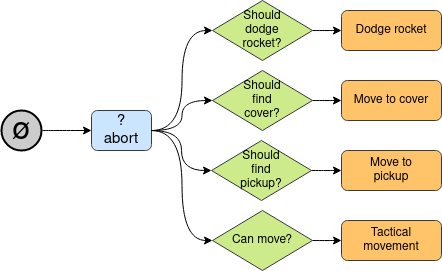
\includegraphics[scale=0.45]{Images/images/FightMovement.drawio.png}} 

\subfloat[\centering Camera and guns]{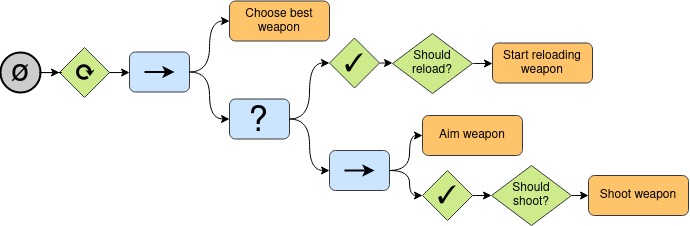
\includegraphics[scale=0.45]{Images/images/FightHead.drawio.png}}
\caption{Behaviour Trees governing the actions of the bot fighting an enemy}
\label{fig:fight_bt}
\end{figure}

A bot enters the \textit{Fight} state whenever it detects the enemy and is in a good enough shape to be able to likely survive the combat.
Correctly handling a fight is a complex process in which the bot must carefully orchestrate how to move, where to move, what weapon should be used, when should it be used or reloaded, as shown in \Cref{fig:fight_bt}.

\paragraph{Movement}\mbox{}\\
For what concerns movement, we identified 4 different objectives:

\begin{enumerate}
\item \textbf{Dodge rockets}: If the bot sees any incoming explosive projectile, it should try to distance itself from the missile and the blast it will cause.
\item \textbf{Find cover}: whenever the bot is running out of ammo and switching weapon might not be convenient, there is a random chance (to avoid predictable behaviors) it might consider moving behind cover to safely reload. If so, the bot find any position from which the enemy cannot see it, move towards that location and stay there until it has finished reloading. If at any point the cover should stop being valid, a new cover point will be selected.
\item \textbf{Collect pickup}: Whenever a useful pickup is close by, the bot can decide go fetch it without abandoning the fight (by avoiding to switch to the Collect pickup state). 
\item \textbf{Keep distance}: The bot will move around trying to try to keep the optimal distance from the enemy based on the currently equipped weapon and, if possible, will try to keep the enemy is sight. More skilled bots will try to circle strafe\footnote{Circle strafing is the technique of moving around an opponent in a circle while facing them. Circle strafing allows a player to fire continuously at an opponent while evading their attacks.} the enemy to gain the upper hand in the fight.
\end{enumerate}

The objective above are ordered by priority, so, for example, dodging rockets will always be preferred over collecting a pickup and, should the enemy fire with such projectile in our direction, we will abort fetching whatever object we wanted to try and dodge the incoming missile.

\paragraph{Gun selection}\mbox{}\\
A bot that simply moves during fight doesn’t achieve much, so for what concerns fighting back the process starts by choosing the optimal weapon to equip.

The gun selection process of the bot involves evaluating two key factors: the distance to the enemy and the amount of available ammo. Based on these parameters, the bot chooses the best weapon for the current combat situation, taking into account the optimal range of each weapon and avoiding, if possible, weapons that require reloading, since it might take a while before the bot is able to use them once equipped. The weapon scored higher according to these criteria is immediately equipped and will be used until another, more suitable weapon, should be chosen instead.

\paragraph{Aiming model}\mbox{}\\
Following the selection of the optimal gun, the bot should try to aim at the target. Although the concept of aiming for a bot is straightforward (just align the cross-hair to the enemy), achieving realistic aiming is more challenging. To account for human-like reaction times and aiming errors, the bot implements a modified version of Arnaboldi's aiming model based on "reflex" and movement predictability, described in \citep{arnaboldi_framework}. 

The bot aims at the enemy's predicted position, taking into account two types of \textit{aiming delays}: an uncorrectable delay and a correctable delay. The correctable delay can be compensated by considering the target's average position in the past. This means that enemy bots with predictable movement patterns will be easier to target than those with erratic movements.

In order to obtain an enemy position and average velocity at a given time, the \textit{Position Tracker} component is used. A \textit{Position Tracker} keeps track of the position of an entity  for every frame in the game up to a given number of seconds in the past. This list of position can be queried to extract both the bot position at a specific time and the bot average velocity in a given range, weighted in order to give less and less importance to velocities far away in time using \Cref{eq:average_velocity}.

\begin{equation}
\overline{v} = \frac{\sum_{i=1}^{n} v_i \cdot \left( W^{t_{end,i} - T_{f}} - W^{t_{start,i} - t_{TF}} \right)}{ \left( W^{T_{f} - T_{i}} \right)} 
\label{eq:average_velocity}
\end{equation}

Where:
\begin{itemize}
\item[$T_i$] The begin of the time range considered.
\item[$T_f$] The end of the time range considered.
\item[$n$] The number of frames for which we recorded position data in the time range considered. Each frame represents an interval of time.
\item[$v_i$] is the velocity in the interval $i$\footnote{Computed as the difference of position between two consecutive frames and the duration between them with the formula: $v_i = \frac{p_{t_{end,i}} - p_{t_{start,i}}}{t_{end,i} - t_{start_i}}$
}
\item[$W$] The weight parameter, the higher it is, the less weight is given to old speeds.
\end{itemize}

In addition to the \textit{aiming delays}, bots have also an \textit{aiming error}: a simple angle representing the deviation from the desired aiming position and the actual one.

\subsubsection{Actuator layer}
%TODO
Every kind of interaction that the bot wants to perform in the virtual world must be processed by the \textit{Actuator layer}, which is currently responsible of moving the bot, rotating the camera or shooting, reloading and switching weapons as a response to what action plan the \textit{decision layer} is currently following.

\subsection{Bot parametrization and profiles}
To emulate different types of human players with varying skills and attitudes, the bot capabilities and behaviors are determined by a set of parameters.

These parameters follow the same principles introduced by Arnaboldi in Cube 2\cite{arnaboldi_framework}, so we defined a \textit{general ability level} affecting all the bot capabilities, and more specific skills that determine a bot proficiency in a particular area compared to other bots with the same general ability level.
In general, the final value for a skill is computed as:

\begin{equation}
skill\_value = min(ability\_score * skill\_score, 1.0)
\label{eq:skill_value}
\end{equation}

The specific characteristics we identified are:
%TODO better ordering
\begin{itemize}
\item \textit{Eye speed}: Determines the maximum camera rotation speed and acceleration. Higher values allow bots to more quickly look in any direction, giving them advantages in scouting an area or aiming at a target.
\item \textit{Reflexes}: Determines how quickly an entity reacts to inputs from the outside world, such as sound for a gun firing, receiving damage or seeing an enemy. 
\item \textit{Prediction skill}: Determines how proficient a bot is in tracking down a lost enemy. Higher values ensure that a bot is more likely to correctly predict an unseen enemy current location.
\item \textit{Aiming skill}: Determines how big the aiming delays and errors are on average, therefore influencing the accuracy of the bot.
\item \textit{Speed}: Determines the movement speed of a bot\footnote{For the purpose of our research, all bots are given the same speed.}.
\item \textit{Movement skill}: Determines how good the bot is in moving tactically when fighting. Higher values ensure a bot employes advanced techniques such as strafing\footnote{Circle strafing is the technique of moving around an opponent in a circle while facing them. Circle strafing allows a player to fire continuously at an opponent while evading their attacks}.
\item \textit{Curiosity}:  The frequency with which the bot looks around instead of solely forward.
\item \textit{Recklessness}: Determines how aggressiveness of the bot. At higher values, a bot will tend to favour combat above everything else, while at low value a bot will prefer finding cover and retreating when in danger.
\item \textit{Field of view}: Determines the field of view of the bot.
\item \textit{Max view range}: The maximum distance an item or enemy can be seen.
\end{itemize}

Using these characteristics, we defined three different bot profiles that will be used in our experiments:
\begin{itemize}
\item \textbf{Shotgun}: The \textit{Shotgun} profile represents a bold and aggressive player who is always ready for a fight. This bot excels in movement, able to quickly close the gap between it and its enemy in order to overpower it in close-quarters combat using its shotgun.
\item \textbf{Sniper}: The \textit{Sniper} profile represents a calculated and patient player who excels in long-range combat. This bot possesses exceptional aiming skills with its sniper rifle, allowing it to take out enemies from a distance with deadly accuracy. It prefers to avoid direct confrontation whenever possible and instead chooses to pick off its enemies from a safe distance. 
\item \textbf{Assault}: The \textit{Assault} profile represents a versatile and well-rounded player who is skilled in both short and medium-range combat. This bot is equipped with an assault rifle.  
\end{itemize}

In \Cref{table:1} the different skills scores for each profile are presented.

%TODO same ordering as above
\begin{table}
\begin{center}
\begin{tabular}{|| c || c | c | c ||}
 \hline
 Skill & Shotgun & Assault & Sniper \\ 
 \hline 
 Eye speed & 1.2 & 1 & 0.8 \\  
 Reflex & 0.9 & 1 & 1.3 \\   
 Prediction & 1.1 & 1 & 0.7 \\  
 Aim & 0.6 & 1 & 1.15 \\  
 Movement & 1.2 & 1 & 0.6 \\  
 Curiosity & High & Neutral & Low \\  
 Recklessness & High & Neutral & Low \\  
 MaxRange & 50 & 120 & 200 \\  
 Speed & 20 & 20 & 20 \\  
 \hline
\end{tabular}
\caption{Different bot profiles defined for our experiments}
\label{table:1}
\end{center}
\end{table}

\section{Summary}
In this chapter we gave a brief overview of Ballabio's Unity Framework, on top of which we built our work.

We then briefly described the kind of data that the framework can gather and analyse during simulation to support any kind of experiment.

Finally, we analyzed the bot system we created to help us run simulations, focusing on its structure and components, how information flows between them, how it makes decisions, what are the parameters governing its decisions and actions and how they can be configured to better represent specific player's capabilities and play styles.

\chapter{Experiments with the framework}
The purpose of this chapter is to test our framework.
We start by better defining the concept of \textit{balance} for the purpose of our research and by ensuring that the bot profiles defined and the weapons they use are balanced.
We then proceed to describe a new map representation, \textit{Grid-graph}, that will be used as a possible replacement for \textit{All-black}.

Using this new representation, we will run some evolutionary experiments with the purpose of obtaining maps capable of restoring balance in a situation of skill gap between players.

\label{section:bot_balance}
\section{Bot balance}

In order to use the profiles defined in the previous chapters for the experiments, we first have to verify that they are \textit{balanced}. Defining what balanced means isn't trivial, and requires defining a context. Consider for example a match between an extremely skilled \textit{Sniper} versus a rookie \textit{Shotgun}. What would be a \textit{balanced} result for a match? An equal number of kills and deaths for the bots might \textit{seem} balanced, but what if the map consists only of long, narrow corridors? In such scenarios, greatly favouring a sniper profile, it would be extremely suspicious if a weak shotgun profile were able to obtain a 1/1 kill-death ratio, hinting that the profiles aren't probably balanced.

\begin{figure}[hbtp]

\centering
\begin{subfigure}[t]{0.3\textwidth}
	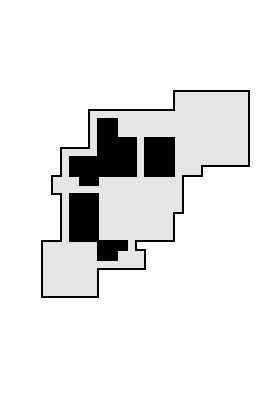
\includegraphics[width=\linewidth]{Images/images/heatmaps/map_generic.png}
	\label{fig:generic_map}
	\caption{The generic map.}
\end{subfigure}
~
\centering
\begin{subfigure}[t]{0.3\textwidth}
	
\includegraphics[width=\linewidth]{Images/images/heatmaps/map_corridor.png}
	\label{fig:corridor_map}
	\caption{The corridor map.}
\end{subfigure}
~
\centering
\begin{subfigure}[t]{0.3\textwidth}
	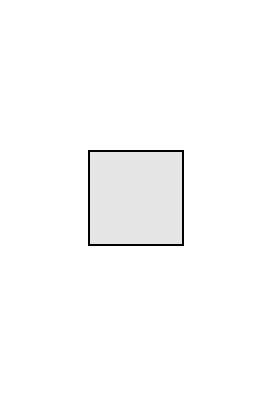
\includegraphics[width=\linewidth]{Images/images/heatmaps/map_arena.png}
	\label{fig:arena_map}
	\caption{The arena map.}
\end{subfigure}
~
\caption{Maps used for our balancing experiments.}
\end{figure}

Given this considerations and the fact that, unlike Arnaboldi and Cube 2 \citep{arnaboldi_framework}, we do not have any pre-made and pre-tested map to use, we opted to test our profiles on three different maps:
\begin{itemize}
\item \textbf{Generic}: A generic map offering oppurtunities for both close, mid and long ranged combats (\Cref{fig:generic_map}).
\item \textbf{Corridor}: A map favouring long-range combat taken to the extreme, consisting of an extremely linear map with no space to dodge projectiles (\Cref{fig:arena_map}).
\item \textbf{Arena}: A map favouring close-range combat taken to the extreme, consisting of a single arena (\Cref{fig:arena_map}).
\end{itemize}

Figures \ref{fig:begin_balance_heatmaps} to \ref{fig:end_balance_heatmaps} show the result of our balance analysis through the use of heatmaps, representing the kill ratio (expressed as \textit{log2}) and absolute kill difference between the two profiles. 
For every matchup, we run different simulations changing the general skill parameter of the two profiles in steps of 0.025.

\subsection{Same profile balance}
Here we show the fight balance for fights between bots with the same profile, but different skill score, on the \textit{generic} map. This can help us validate that changing the skill score has a tangible effect on the capabilities of the bot.

\begin{figure}[H]
    \centering
    \begin{subfigure}[t]{0.5\textwidth}
        \centering
        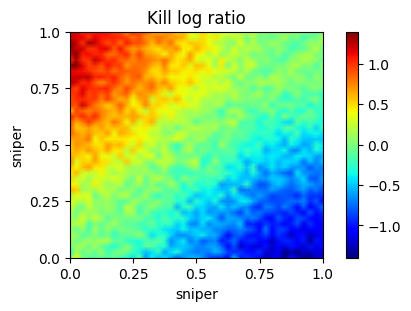
\includegraphics[height=5cm]{Images/images/heatmaps/same-profile/sniper_heatmap_ratio.png}
    \end{subfigure}%
    ~ 
    \begin{subfigure}[t]{0.5\textwidth}
        \centering
        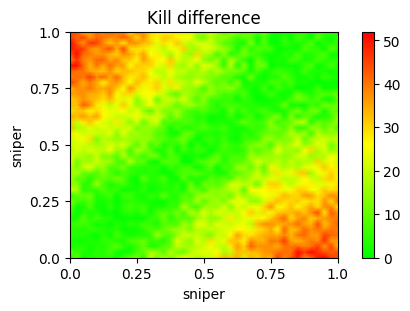
\includegraphics[height=5cm]{Images/images/heatmaps/same-profile/sniper_heatmap_diff.png}
    \end{subfigure}
    \caption{Heatmaps for the \textit{Sniper} vs \textit{Sniper} matchup.}
    \label{fig:balance_sniper_sniper}
    \label{fig:begin_balance_heatmaps}
\end{figure}

\begin{figure}[H]
    \centering
    \begin{subfigure}[t]{0.5\textwidth}
        \centering
        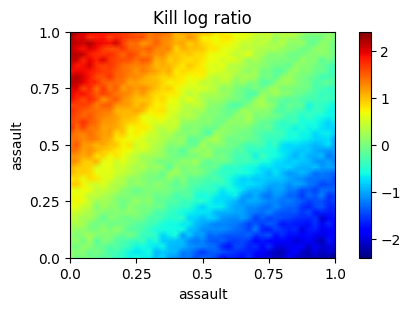
\includegraphics[height=5cm]{Images/images/heatmaps/same-profile/assault_heatmap_ratio.png}
    \end{subfigure}%
    ~ 
    \begin{subfigure}[t]{0.5\textwidth}
        \centering
        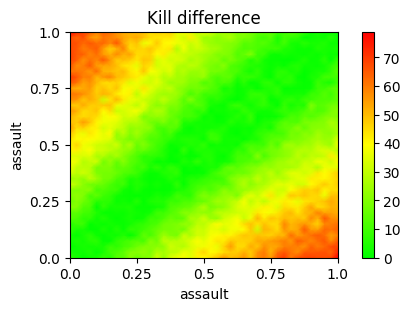
\includegraphics[height=5cm]{Images/images/heatmaps/same-profile/assault_heatmap_diff.png}
    \end{subfigure}
    \caption{Heatmaps for the \textit{Assault} vs \textit{Assault} matchup.}
    \label{fig:balance_assault_assault}
\end{figure}

\begin{figure}[H]
    \centering
    \begin{subfigure}[t]{0.5\textwidth}
        \centering
        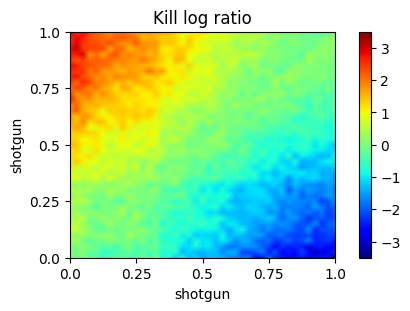
\includegraphics[height=5cm]{Images/images/heatmaps/same-profile/shotgun_heatmap_ratio.png}
    \end{subfigure}%
    ~ 
    \begin{subfigure}[t]{0.5\textwidth}
        \centering
        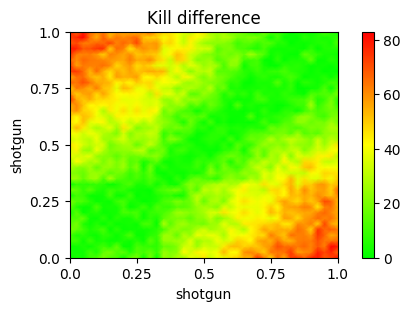
\includegraphics[height=5cm]{Images/images/heatmaps/same-profile/shotgun_heatmap_diff.png}
    \end{subfigure}
    \caption{Heatmaps for the \textit{Shotgun} vs \textit{Shotgun} matchup.}
    \label{fig:balance_shotgun_shotgun}
\end{figure}

From this first balancing experiment we can verify that changing the \textit{general skill} has a noticeable effect on the capabilities of the bot and bots with higher general skill are able to achieve better results against lower skilled opponents.
We can also notice how the \textit{Shotgun} profile is the most influenced by the skill parameter, since it is the one capable of achieving the highest kill ratio and absolute kill difference. This is likely related to the fact that the \textit{Shotgun} is the weapon with the highest \textit{Damage Per Second} in the game and it is therefore capable, in the right hand, to score more kills in the time allotted. Conversely, the \textit{Sniper} is the one showing the smallest difference between skilled and unskilled player, probably for similar reasons.

\subsection{Arena map balance}

In the \textit{Arena} map, as expected, the \textit{Shotgun} profile is the one capable of achieving the best results against the other two profiles, managing to hold its ground even when fighting stronger opponents in terms of skill.

We can also notice how the \textit{Sniper} profile isn't able to shine particularly, not even at the highest levels of skill, as expected due to the limited size of the map.

\begin{figure}[H]
    \centering
    \begin{subfigure}[t]{0.5\textwidth}
        \centering
        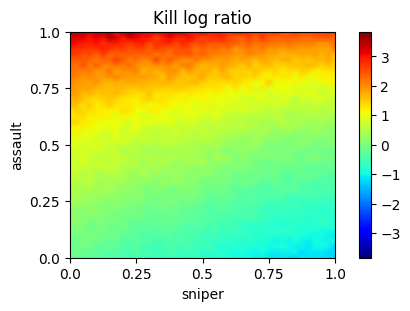
\includegraphics[height=5cm]{Images/images/heatmaps/short-range/assault_sniper_heatmap_ratio.png}
    \end{subfigure}%
    ~ 
    \begin{subfigure}[t]{0.5\textwidth}
        \centering
        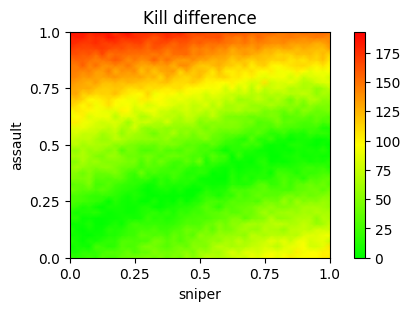
\includegraphics[height=5cm]{Images/images/heatmaps/short-range/assault_sniper_heatmap_diff.png}
    \end{subfigure}
    \caption{Heatmaps for the \textit{Assault} vs \textit{Sniper} matchup.}
    \label{fig:balance_assault_sniper_short}
\end{figure}

\begin{figure}[H]
    \centering
    \begin{subfigure}[t]{0.5\textwidth}
        \centering
        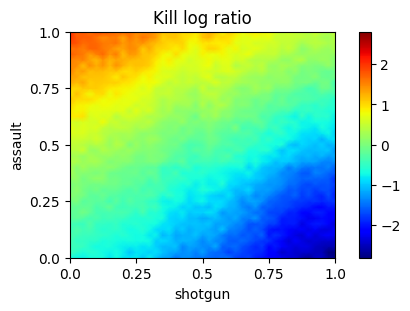
\includegraphics[height=5cm]{Images/images/heatmaps/short-range/assault_shotgun_heatmap_ratio.png}
    \end{subfigure}%
    ~ 
    \begin{subfigure}[t]{0.5\textwidth}
        \centering
        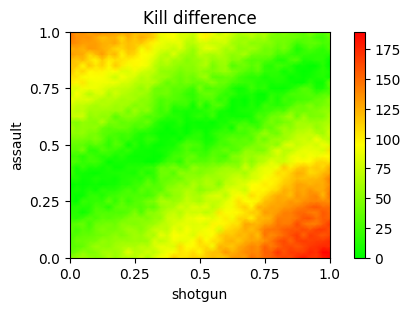
\includegraphics[height=5cm]{Images/images/heatmaps/short-range/assault_shotgun_heatmap_diff.png}
    \end{subfigure}
    \caption{Heatmaps for the \textit{Assault} vs \textit{Shotgun} matchup.}
    \label{fig:balance_assault_shotgun_short}
\end{figure}

\begin{figure}[H]
    \centering
    \begin{subfigure}[t]{0.5\textwidth}
        \centering
        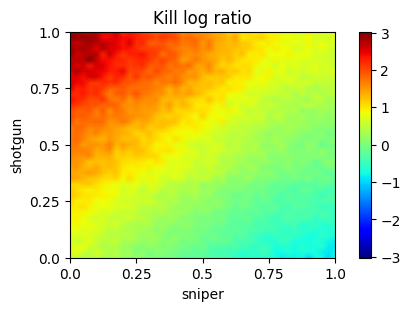
\includegraphics[height=5cm]{Images/images/heatmaps/short-range/shotgun_sniper_heatmap_ratio.png}
    \end{subfigure}%
    ~ 
    \begin{subfigure}[t]{0.5\textwidth}
        \centering
        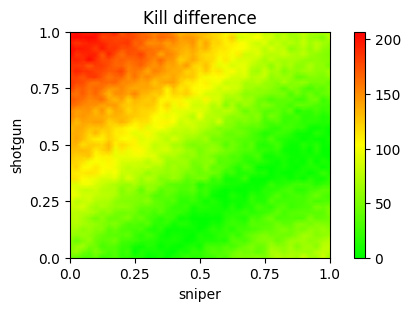
\includegraphics[height=5cm]{Images/images/heatmaps/short-range/shotgun_sniper_heatmap_diff.png}
    \end{subfigure}
    \caption{Heatmaps for the \textit{Shotgun} vs \textit{Sniper} matchup.}
    \label{fig:balance_shotgun_sniper_short}
\end{figure}

\subsection{Generic map balance}
For the \textit{Generic} map, we can see that the situation is more or less balanced for all matchups, except the \textit{Sniper} vs \textit{Shotgun} matchup which shows a little disadvantage for the \textit{Sniper}. This doesn't necessarily mean that the \textit{Sniper} profile is weaker in general, the map might be favouring slightly the \textit{Shotgun}.

\begin{figure}[H]
    \centering
    \begin{subfigure}[t]{0.5\textwidth}
        \centering
        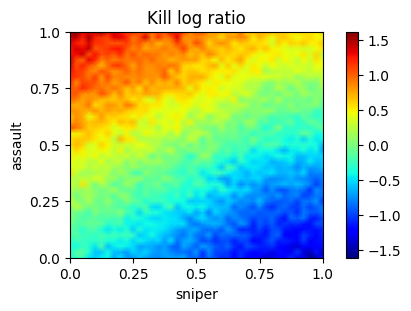
\includegraphics[height=5cm]{Images/images/heatmaps/mid-range/assault_sniper_heatmap_ratio.png}
    \end{subfigure}%
    ~ 
    \begin{subfigure}[t]{0.5\textwidth}
        \centering
        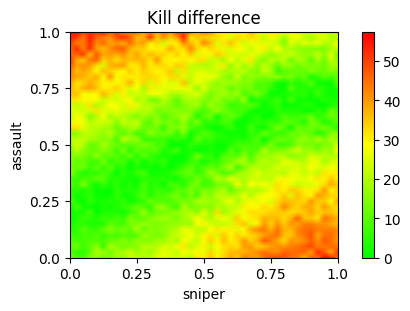
\includegraphics[height=5cm]{Images/images/heatmaps/mid-range/assault_sniper_heatmap_diff.png}
    \end{subfigure}
    \caption{Heatmaps for the \textit{Assault} vs \textit{Sniper} matchup.}
    \label{fig:balance_assault_sniper_mid}
\end{figure}

\begin{figure}[H]
    \centering
    \begin{subfigure}[t]{0.5\textwidth}
        \centering
        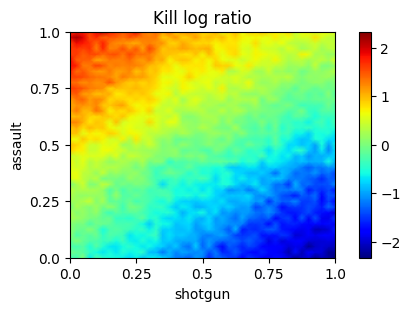
\includegraphics[height=5cm]{Images/images/heatmaps/mid-range/assault_shotgun_heatmap_ratio.png}
    \end{subfigure}%
    ~ 
    \begin{subfigure}[t]{0.5\textwidth}
        \centering
        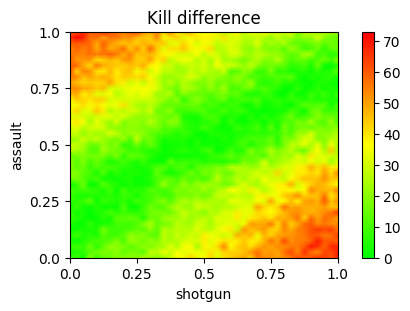
\includegraphics[height=5cm]{Images/images/heatmaps/mid-range/assault_shotgun_heatmap_diff.png}
    \end{subfigure}
    \caption{Heatmaps for the \textit{Assault} vs \textit{Shotgun} matchup.}
    \label{fig:balance_assault_shotgun_mid}
\end{figure}

\begin{figure}[H]
    \centering
    \begin{subfigure}[t]{0.5\textwidth}
        \centering
        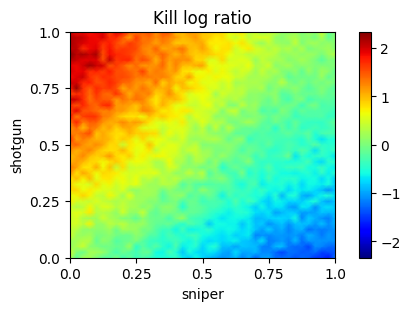
\includegraphics[height=5cm]{Images/images/heatmaps/mid-range/shotgun_sniper_heatmap_ratio.png}
    \end{subfigure}%
    ~ 
    \begin{subfigure}[t]{0.5\textwidth}
        \centering
        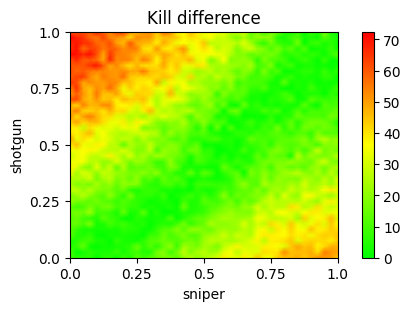
\includegraphics[height=5cm]{Images/images/heatmaps/mid-range/shotgun_sniper_heatmap_diff.png}
    \end{subfigure}
    \caption{Heatmaps for the \textit{Shotgun} vs \textit{Sniper} matchup.}
    \label{fig:balance_shotgun_sniper_mid}
\end{figure}

%###############

\subsection{Corridor map balance}

Finally, in the \textit{Corridor} map, we can see, as expected, that the \textit{Sniper} profile is able, even at the lowest skill level, to defeat the other two profiles and, in the matchup against the \textit{Shotgun}, by a wide margin,
Interestingly enough however, the \textit{Assault} rifle is the one capable of achieving the best kill ratio (8/1) against the \textit{Shotgun} profile. This is likely caused by the higher DPS of the \textit{Assault} rifle, which allows the wielder to dispatch opponents faster.

\begin{figure}[H]
    \centering
    \begin{subfigure}[t]{0.5\textwidth}
        \centering
        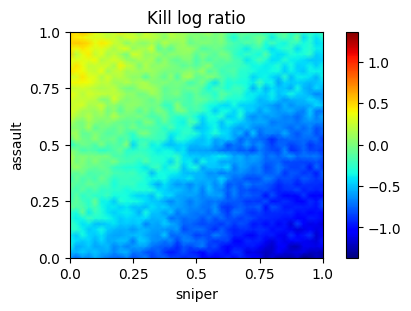
\includegraphics[height=5cm]{Images/images/heatmaps/long-range/assault_sniper_heatmap_ratio.png}
    \end{subfigure}%
    ~ 
    \begin{subfigure}[t]{0.5\textwidth}
        \centering
        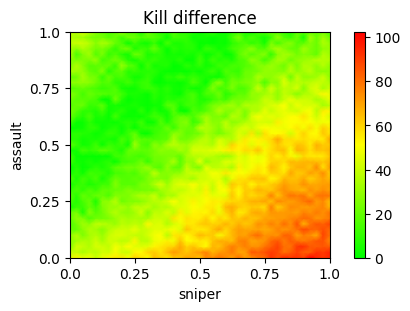
\includegraphics[height=5cm]{Images/images/heatmaps/long-range/assault_sniper_heatmap_diff.png}
    \end{subfigure}
    \caption{Heatmaps for the \textit{Assault} vs \textit{Sniper} matchup.}
    \label{fig:balance_assault_sniper_long}
\end{figure}

\begin{figure}[H]
    \centering
    \begin{subfigure}[t]{0.5\textwidth}
        \centering
        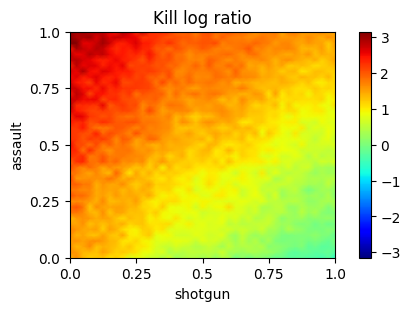
\includegraphics[height=5cm]{Images/images/heatmaps/long-range/assault_shotgun_heatmap_ratio.png}
    \end{subfigure}%
    ~ 
    \begin{subfigure}[t]{0.5\textwidth}
        \centering
        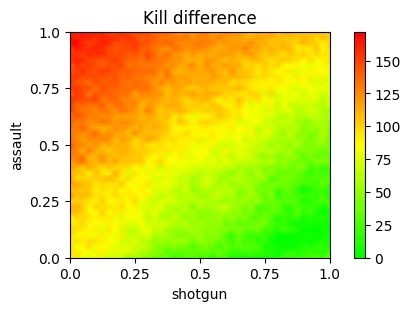
\includegraphics[height=5cm]{Images/images/heatmaps/long-range/assault_shotgun_heatmap_diff.png}
    \end{subfigure}
    \caption{Heatmaps for the \textit{Assault} vs \textit{Shotgun} matchup.}
    \label{fig:balance_assault_shotgun_long}
\end{figure}

\begin{figure}[H]
    \centering
    \begin{subfigure}[t]{0.5\textwidth}
        \centering
        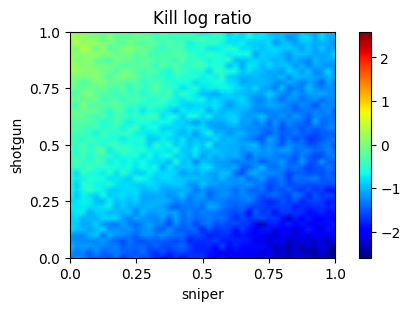
\includegraphics[height=5cm]{Images/images/heatmaps/long-range/shotgun_sniper_heatmap_ratio.png}
    \end{subfigure}%
    ~ 
    \begin{subfigure}[t]{0.5\textwidth}
        \centering
        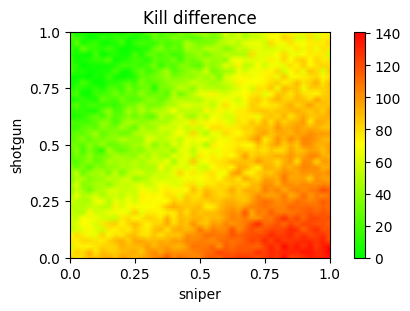
\includegraphics[height=5cm]{Images/images/heatmaps/long-range/shotgun_sniper_heatmap_diff.png}
    \end{subfigure}
    \caption{Heatmaps for the \textit{Shotgun} vs \textit{Sniper} matchup.}
    \label{fig:balance_shotgun_sniper_long}
    \label{fig:end_balance_heatmaps}
\end{figure}

\section{Grid-graph map representation}
In this section we describe the original \textit{All-black} representation used in the framework, analyse some of its shortcomings and propose a new representation \textit{Grid-graph}, on top of which the different evolutionary experiments will be run.

\subsubsection{Limits of the original models}
Many of the researches performed on evolution of maps for first person shooter used as their basis the map genotypes developed by Cardamone \citep{cardamone_evolving_maps}. Among the four proposed representations, \textit{Grid}, \textit{All-white}, \textit{All-black} and \textit{Random-Digger}, \textit{All-white} was the one capable of producing the maps with the highest fitness, but the produced result look bland and lack any notable feature.
The \textit{All-black} representation on the other hand, despite performing worse on average, managed to create maps which strongly resemble those produced by level designer, thanks to their emphasis on arenas and corridors, and was therefore chosen as the basis for other researches, such as Arnaboldi's \citep{arnaboldi_framework}. 

We have analysed the \textit{All-black} representation to try to understand why it under performed in the settings of an evolutionary algorithms with exploration of the search space and found two major problems.

The first of this problems is the \textbf{redundancy}. \Cref{fig:all_black_connected} shows an example of the problem: in this genotype, one of the rooms, specifically \textit{<4,3,2>}, is redundant, since it's completely contained in room \textit{<4,4,4>}. Only considering these two rooms, the smallest one can be placed in 8 other positions and still have no effect on the final phenotype. This redundancy problem leads to an exponential increase in the size of the search space, which in turn slows down convergence of any search algorithm employed.

The second problem is the \textbf{lack of locality}, two very similar genotypes can produce substantially different phenotypes, making it difficult for the exploration algorithm to understand how to optimize the fitness function. An example of this phenomenon is presented in \Cref{fig:all_black_disconnected}: a map obtained by simply changing two numbers of the genotype represented in \Cref{fig:all_black_connected}. While one of the changes leads to a negligible variation in the phenotype, the other completely alters the connectivity of the map, greatly affecting the way the map is played.

\begin{figure}
\centering
\captionsetup[subfigure]{}
\subfloat[\centering All-black initial representation]{
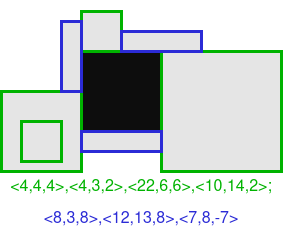
\includegraphics[scale=0.7]{Images/images/ABConnected.png}
\label{fig:all_black_connected}
} 
\subfloat[\centering All-black representation after two small changes]{
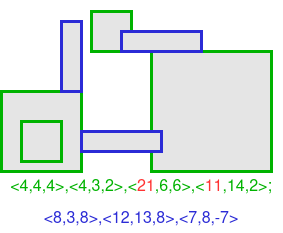
\includegraphics[scale=0.7]{Images/images/ABDisconnected.png}
\label{fig:all_black_disconnected}
} 

\caption{Examples of two All-black representations}
\end{figure}

\subsection{Graph-based map representation: Grid-graph}
In this thesis we propose a graph-based genotype representation for maps, named \textit{Grid-graph}, which should overcome the limitations of the \textit{All-black} representation while still maintaining a lot of similarities and ease of use. 

The \textit{Grid-graph} map representation follows the same approach used by \textit{All-black} and starts with an initial map full of wall blocks and gradually adds space in search of fitter maps.

To place free space, \textit{Grid-graph} starts by subdividing the area into an $R \times C$ grid of equally sized cells, each one occupying $r \times c$ squares. A cell contains zero or one \textbf{Room}, representing a rectangular, axis-aligned, walkable portion of the map. Each room is defined by four values:
\begin{itemize}
\item[w] The width of the \textit{Room}, between 1 and $c$.
\item[h] The height of the \textit{Room}, between 1 and $r$.
\item[x] The x coordinate of the bottom left corner of the \textit{Room} inside the cell, between 0 and $c-w-1$. 
\item[y] The y coordinate of the bottom left corner of the \textit{Room} inside the cell, between 0 and $r-h-1$.
\end{itemize}
To represent the contents of each cell, the genome contains an $R \times C$ matrix where element $(i,j)$ contains the quartet described above if the cell in position $(i,j)$ contains a \textit{Room} or a special value \textit{Nil} in case no \textit{Room} is placed in that cell\footnote{It is possible for this genome to represent maps which do not contain any free space. When that happens, the genome should simply be discarded.}.

\textit{Rooms} placed in vertically or horizontally adjacent cells can be connected by a \textbf{Corridor}. Each corridor is simply represented as a boolean value \textit{<b>} indicating whether the two adjacent rooms (if present) must be connected. All the horizontal corridors are saved in a $R \times (C-1)$ matrix, where the boolean at position $(i,j)$ represents whether \textit{Rooms} $(i,j)$, $(i,j+1)$ are connected and similarly all the vertical corridors are stored in an $(R-1) \times C$ matrix, where the boolean at position $(i,j)$ represents whether \textit{Rooms} $(i,j)$, $(i+1,j)$ are connected.

\textit{Corridors} do not have any specified size or shape defined in the genotype, rather, they are generated dynamically to connect the various rooms depending on the placement of them. For example, two rooms which are not aligned must be connected by a corridor with a bend in the middle, or again, two rooms adjacent by at least one square do not need a corridor at all and are simply fused together. 

When converting the genome to it's actual map representation, it possible to run into a problem: the resulting map might be disconnected. This problem was already identified by Cardamone \cite{cardamone_evolving_maps} for other map representations and we will be using the same approach adopted in his research: in case of multiple disjointed connected components, the one closest to the center is selected and the other parts of the map are ignored.

An example of \textit{Grid-graph} genome and related phenotype are shown in \Cref{fig:grid-graph-genome-phenotype}.

\begin{figure}[hbtp]
\centering
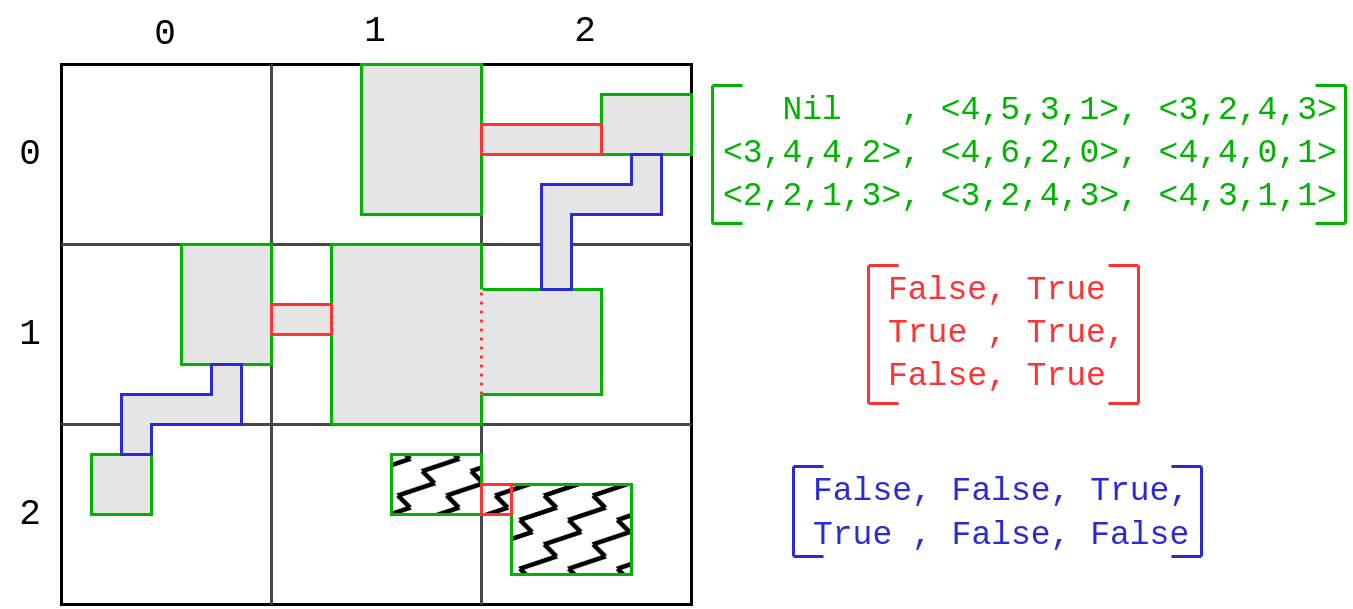
\includegraphics[width=0.9\linewidth]{Images/images/Grid-graph.png}
\caption{Example of Grid-graph phenotype and related genotype. \textcolor{green}{Rooms} are shown in green, \textcolor{red}{horizontal corridors} in red and \textcolor{blue}{vertical corridors} in blue. The parts of the map disconnected are filled with a zig-zagged line}
\label{fig:grid-graph-genome-phenotype}
\end{figure}

\begin{figure}
\centering
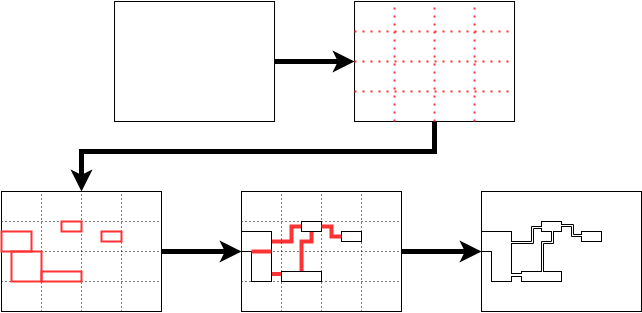
\includegraphics[scale=0.6]{Images/images/MapGeneration.drawio.png}  
\caption{Generation process for a Grid-graph map}
\label{fig:grid-graph-generation}
\end{figure}

\subsubsection{Comparison between All-black and Grid-graph}
The \textit{Grid-graph} map representation tries to maintain some of the key concepts used in the \textit{All-black} representation and refines others. 

\textit{Rooms} for example are virtually identical between the two representations and the most notable difference is that in \textit{Grid-graph} their placement is not completely free, since each room must be placed in a cell and only one \textit{Room} can be contained in each cell.

\textit{Corridors} instead have been completely revamped: while in \textit{All-black} a corridor is just a non-square room, in \textit{Grid-graph} corridors have a proper function: connecting different rooms. This greatly simplifies maps, since connecting non-aligned rooms doesn’t require strategically placed corridors as was the case for \textit{All-black}, and make maps more resilient to changes since now two rooms cannot get disconnected by chance, simply because they got resized or moved.

Since \textit{Rooms} and \textit{Corridors} in \textit{Grid-graph} map can be placed only in specific places and overlaps are forbidden, this representation does not incur in same kind of \textit{redundancy} problem prominent in \textit{All-black} maps. 
However, it should be noted that, given the grid layout of \textit{Grid-graph}, maps will tend to look more simple than those obtained with \textit{All-Black}. As an example, consider the map in \Cref{fig:complex_AB_map}. It would be basically impossible for \textit{Grid-graph} to replicate many of the features, such as little nooks and crannies, dead-end corridors, extra walls and so on.
Nonetheless, it's not clear yet the influence that all those little features have on matches, they could be an integral part in what makes a given map great or they could simply be considered "noise" that can be simply discarded.

Regarding the second problem present in \textit{All-black} maps instead, the \textit{lack of locality}, \textit{Grid-graph} maps are also affected by it, but in a more controllable way, since two adjacent regions of the map can be disconnected only if the room or corridor connecting them is removed. With \textit{All-black} instead any modification to any parameter can potentially alter the map topology, be it moving, removing or resizing a room or corridor.

\begin{figure}
\centering
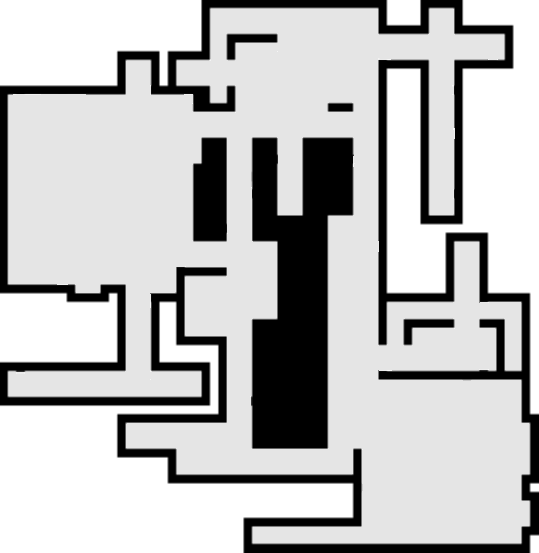
\includegraphics[scale=0.4]{Images/images/random-arnaboldi-map.png}  
\caption{Example of map obtained using All-black representation}
\label{fig:complex_AB_map}
\end{figure}

\section{Evolving new maps: Balance and pacing}
For this experiment we wanted to evolve maps which, starting from a initial situation of unbalance due to the different level of skill of the players involved, tries to evolve maps that result in balanced matches, additionally trying to maximize the \textit{pace}.
We will be running the experiment in two different configurations, one using the \textit{Grid-graph} representation and the other using the \textit{All-black} representation, in order to compare the two. For each experiment we will be executing 8 different runs.

\subsection{Common setup}

The two experiments we will conduct have several parameters in common, starting with the profiles used: \textit{Sniper} and \textit{Shotgun}, summarised in \Cref{table:parameters_first_experiment}, and their respective skill levels of 0.15 and 0.85. For this combination of profiles and skills, the resulting entropy achieved in the experiments conducted on the generic map in in \Cref{section:bot_balance} was approximately 0.84, corresponding to a kill ratio of 2.77 in favour of the \textit{Shotgun}.

\begin{table}
\begin{center}
\begin{tabular}{|| c || c | c ||}
 \hline
 Skill & Shotgun & Sniper \\ 
 \hline 
 Eye speed & 1.2 & 0.8 \\  
 Reflex & 0.9 & 1.3 \\   
 Prediction & 1.1 & 0.7 \\  
 Aim & 0.6 & 1.15 \\  
 Movement & 1.2 & 0.6 \\  
 Curiosity & High & Low \\  
 Recklessness & High & Low \\  
 Max Range & 50 & 200 \\  
 Speed & 20 & 20 \\  
 \hline
\end{tabular}
\caption{Different bot profiles defined for our experiments}
\label{table:parameters_first_experiment}
\end{center}
\end{table}

Both experiments will involve populations consisting of 52 individuals, spanning across 30 generations, and will utilize a multi-objective fitness approach in conjunction with the NSGA-II selection algorithm \cite{ngsaII}. 

Any time the algorithm needs to run a match between the bots, two game simulations, lasting 20 minutes each, are launched and the final results, used to compute the fitness, are averaged. This was done in order to reduce any potential error caused by the stochastic nature of the bots and of the simulations.

\subsection{Grid-graph experiment}
For our first experiment, we will test how suitable the \textit{Grid-graph} representation is in the context of evolutionary algorithms.

We will use a map composed of an 8x8 grid of cells, evolved using as \textit{crossover} operation a simple matrix crossover (given the grid nature of the map) with probability $0.3$ and as \textit{mutation} operator a two-points mutation with probability 0.3.

\Cref{fig:ex_one_pareto_area} shows the evolution of the area under the Pareto front for the first 30 generations of the evolutionary process, averaged across the runs.
Looking at the picture, we can observe a continuous expansion of the Pareto front area during the whole process, but the increase per epoch slows down drastically after the fifteenth generation. Considering the whole process, the average area under the Pareto front grew by 12\%.

\begin{figure}[hbtp]
\centering
\includegraphics[width=0.5\linewidth]{Images/images/experiment_one/Pareto/pareto_evolution_avg.png}
\caption{Evolution of the area under the Pareto front}
\label{fig:ex_one_pareto_area}
\end{figure}

\begin{figure}[hbtp]
    \centering
    \begin{subfigure}[t]{0.5\textwidth}
        \centering
        \includegraphics[height=7cm]{Images/images/experiment_one/Pareto/pareto_front_total_begin.png}
        \caption{Initial Pareto front.}
    \end{subfigure}%
    ~ 
    \begin{subfigure}[t]{0.5\textwidth}
        \centering
        \includegraphics[height=7cm]{Images/images/experiment_one/Pareto/pareto_front_total_final.png}
        \caption{Final Pareto front.}
        \label{fig:ex_one_final_pareto_total}
    \end{subfigure}
    \caption{Evolution of the Pareto front.}
    \label{fig:ex_one_pareto_evolution}
\end{figure}


\begin{figure}[hbtp]
    \centering
    \begin{subfigure}[t]{0.5\textwidth}
        \centering
        \includegraphics[height=7cm]{Images/images/experiment_one/Pareto/pareto_front_population_0.png}
    \end{subfigure}%
    ~ 
    \begin{subfigure}[t]{0.5\textwidth}
        \centering
        \includegraphics[height=7cm]{Images/images/experiment_one/Pareto/pareto_front_population_1.png}
    \end{subfigure}
    \caption{Pareto front of 2 of the 8 runs.}
    \label{fig:ex_one_pareto_populations}
\end{figure}


\Cref{fig:ex_one_pareto_evolution} allows us to compare the Pareto front at the start and end of the evolutionary process. It's evident that there hasn't been a significant increase in \textit{pace}, but in terms of \textit{entropy}, there has been a noticeable shift from a maximum value of approximately 0.9 to a value close to 1 (0.998), or, in terms of kill ratio, a decrease from 2.1 to 1.1.

The unsatisfactory improvements in \textit{pace} can be attributed to a simple consideration: a \textit{pace} value of $0.9$ corresponds to a combat every second, a rate that cannot be further improved due to the time it takes for bots to respawn and react to enemies. 
\Cref{fig:best_pace_map_0} and \Cref{fig:best_pace_map_1} show the best maps, in terms of \textit{pace}, for two of the eight simulations run. These two maps look extremely bland, they just consist of a single room, offering no cover or escape, therefore forcing combat immediately every time.

In contrast, the improvements in \textit{entropy} are much more promising, especially when considering its logarithmic trend. A value of 0.9 corresponds to a kill-death ratio of around $2.2$ in favor of the \textit{Shotgun} profile, while a unitary value indicates a perfect balance between the bots. An almost perfect balance was achieved by the map shown in \Cref{fig:best_entropy_map_0}.

The distribution of values in \Cref{fig:ex_one_final_pareto_total} shows a concentration of individuals having high pace values and average entropy values, but there are also plenty of other individuals scattered around, hinting that a big portion of the search space was explored during the evolution.

Lastly, it's noticeable that while for average \textit{entropy} values the evolutionary algorithm has always been able to find maps that maximize \textit{pace}, with entropy values tending towards 1, there is a sudden reversal of this trend, leading, at the extreme, to a pace value as low as $0.46$. This behavior can be reasonably explained by considering that those maps which maximize \textit{entropy} tend to be highly elongated, increasing the time it takes for bots to find each other and start combat.

%\begin{figure}[hbtp]
%    \centering
%    \begin{subfigure}[t]{0.3\textwidth}
%        \centering
%        \includegraphics[height=4.5cm]{Images/images/experiment_one/best_entropy_total/map.png}
%        \caption{Map with entropy 0.999 and pace 0.689.}
%        \label{fig:ex_one_map_entropy}
%    \end{subfigure}%
%    ~ 
%    \begin{subfigure}[t]{0.3\textwidth}
%        \centering
%        \includegraphics[height=4.5cm]{Images/images/experiment_one/best_fitness_total/map.png}
%        \caption{Map with entropy 0.992 and pace 0.775.}
%    \end{subfigure}
%    ~ 
%    \begin{subfigure}[t]{0.3\textwidth}
%        \centering
%        \includegraphics[height=4.5cm]{Images/images/experiment_one/best_pace_total/map.png}
%        \caption{Map with entropy 0.729 and pace 0.897}
%        \label{fig:ex_one_map_pace}
%    \end{subfigure}
%    \caption{Maps maximising entropy, pace and fitness considering all populations combined.}
%    \label{fig:ex_one_pareto_evolution_combined}
%\end{figure}

\begin{figure}[hbtp]
    \centering
    \begin{subfigure}[t]{0.3\textwidth}
        \centering
        \includegraphics[height=4.5cm]{Images/images/experiment_one/best_entropy_pop_0/map.png}
        \caption{Map with entropy 0.998 and pace 0.611.}
        \label{fig:best_entropy_map_0}
    \end{subfigure}%
    ~ 
    \begin{subfigure}[t]{0.3\textwidth}
        \centering
        \includegraphics[height=4.5cm]{Images/images/experiment_one/best_fitness_pop_0/map.png}
        \caption{Map with entropy 0.981 and pace 0.674.}    
        \label{fig:best_fitness_map_0}
    \end{subfigure}
    ~ 
    \begin{subfigure}[t]{0.3\textwidth}
        \centering
        \includegraphics[height=4.5cm]{Images/images/experiment_one/best_pace_pop_0/map.png}
        \caption{Map with entropy 0.769 and pace 0.869}
        \label{fig:best_pace_map_0}
    \end{subfigure}
    \centering
    \begin{subfigure}[t]{0.3\textwidth}
        \centering
        \includegraphics[height=4.5cm]{Images/images/experiment_one/best_entropy_pop_1/map.png}
        \caption{Map with entropy 0.988 and pace 0.466.}
        \label{fig:best_entropy_map_1}
    \end{subfigure}%
    ~ 
    \begin{subfigure}[t]{0.3\textwidth}
        \centering
        \includegraphics[height=4.5cm]{Images/images/experiment_one/best_fitness_pop_1/map.png}
        \caption{Map with entropy 0.963 and pace 0.749.}
        \label{fig:best_fitness_map_1}
    \end{subfigure}
    ~ 
    \begin{subfigure}[t]{0.3\textwidth}
        \centering
        \includegraphics[height=4.5cm]{Images/images/experiment_one/best_pace_pop_1/map.png}
        \caption{Map with entropy 0.804 and pace 0.876}
        \label{fig:best_pace_map_1}
    \end{subfigure}
    \caption{Maps maximising entropy, fitness and pace considering two of the eight runs.}
    \label{fig:ex_one_maps}
\end{figure}


\subsubsection{Map analysis}
One of the first things that stands out from the displayed maps is the simplicity (not to say banality) of the maps obtained by maximizing pace. It simply consists of one room. On these maps, the high visibility and limited total space result in combat occurring at a very fast and potentially exhausting pace. 

Coincidentally, maps maximing \textit{pace} are those with the lowest \textit{entropy}. This is expected, considering the weapons in play. The \textit{Shotgun} profile in particolar shines in close-range combat and this, coupled with the higher general skill, means that the \textit{Sniper} profile cannot compete.

On the other end of the spectrum, maps that maximize \textit{entropy} feature linear structures that favor long-range combat and limit longitudinal movements, preventing the use of techniques such as strafing to approach enemies while avoiding being hit. Additionally, it is often possible to observe the absence of alternative paths to reach any point on the map, further reducing the possibility of approaching enemy snipers. 

%Finally, when observing maps that maximize \textit{fitness}, it is possible to notice an interesting detail for \Cref{fig:ex_one_map_entropy} and \Cref{fig:ex_one_map_fitness}: the latter can be obtained by stripping away the leftmost part of the former, reducing The structure of the obtained maps more closely resemble that of a single long vertical corridor, which still favours long-range combat but also increases the total visibility, leading to more frequent combats.

\subsubsection{Analysis of the dynamics}
We now proceed to analyse the evolved maps using data gathered by our framework. We will be in particular focusing on:
\begin{itemize}
\item \textbf{Kill and Death Heatmaps}: These graphics will display, for each map, at which points kills and deaths tend to occur more or less frequently.
\item \textbf{Kill traces}: These graphics will display the relative position of bots at each individual kill through a segment whose color will be darker the greater the distance between the two.
\end{itemize} 

These graphics are shown in Figures
\ref{fig:ex_one_begin_heatmaps} to \ref{fig:ex_one_end_heatmaps}.

Except for the maps that maximizes \textit{pace}, which, due to their limited size, do not reveal particularly interesting details on match dynamics, the kill traces of the other maps show two distinct play styles for \textit{Shotgun} and \textit{Sniper} profiles that are reflected in their respective death and kill positions.

In regards to the \textit{Sniper} profile, it is noticeable how kills tend to concentrate in close proximity to walls and in the most extreme positions of the maps, locations that allow the \textit{Sniper} to shoot opponents from a safe distance, but which simultaneously do not provide any possibility of retreat in case of need.

Conversely, the \textit{Shotgun} profile frequently positions itself in the most central and open areas of the maps, taking advantage of its high mobility to close in on opponents while evading incoming fire.

%Looking at the death heatmaps, another interesting observation can be made. While it's expected that deaths are concentrated around the central junctions of the map (simply because it's often necessary to cross them to reach any destination), we can see that \textit{Sniper} deaths are always concentrated in the vicinity, while \textit{Shotgun} deaths are more spread out (this is especially noticeable for the second experiment). This is likely due to the different characteristics of the weapons: as soon as the \textit{Shotgun} profile spots an enemy at a crossroad, they only need a single shot to eliminate them. In contrast, a \textit{Sniper }needs two shots, giving the enemy time to move.

\subsubsection{Relation to other characteristics}
As a final analysis, we wanted to investigate if there were any particular relationships between \textit{entropy} and other characteristics, particularly \textit{pace}, \textit{accuracy}, \textit{sight loss rate} and \textit{number of frags}, across all runs. The results, shown in \Cref{fig:ex_one_entropy_relations}, are not particularly surprising given that the evolutionary process aimed to balance a situation of significant disadvantage for the \textit{Sniper} profile.

We can observe a general increase in the \textit{accuracy} and the number of kills or the \textit{Sniper} profile, while there was a clear decrease in the effectiveness of the \textit{Shotgun}, despite the accuracy remaining rather constant during the process. 

This can be attributed to the shape of the maps, which became increasingly narrow and elongated as \textit{entropy} increased, favoring the \textit{Sniper} profile's accuracy (as the \textit{Shotgun} profile has fewer opportunities to evade bullets) without significantly modifying the \textit{Shotgun}'s accuracy, given that the \textit{Shotgun} is already accurate enough at short distances and the \textit{Sniper} isn't proficient in evading techniques such as \textit{strafing}. The decrease in the number of kills for the \textit{Shotgun} profile follows the reduction in the \textit{pace}, which again is likely caused by their gradual elongation of maps which reduces visibility and engage opportunities.

We can also notice a consistent decrease in \textit{Pace}, which can be attributed to the fact that the \textit{Shotgun} profile prefers smaller and more frenetic maps, whereas the \textit{Sniper} profile prefers longer and more stretched-out maps, which slow down the \textit{pace} of encounters.

% TODO evoluzione area delle mappe?

\begin{figure}[H]
\centering
\includegraphics[width=0.6\linewidth]{Images/images/experiment_one/entropy_mix.png}
\caption{Relation of entropy to other characteristics}
\label{fig:ex_one_entropy_relations}
\end{figure}


\newpage

%BEGIN Shotgun first simulation
\begin{figure}[H]
    \centering
    \begin{subfigure}[t]{0.3\textwidth}
        \centering
        \includegraphics[height=4.5cm]{Images/images/experiment_one/best_entropy_pop_0/deaths_bot_0.png}
        \caption{Map maximising entropy.}
    \end{subfigure}%
    ~ 
    \begin{subfigure}[t]{0.3\textwidth}
        \centering
        \includegraphics[height=4.5cm]{Images/images/experiment_one/best_fitness_pop_0/deaths_bot_0.png}
        \caption{Map maximising fitness.}
    \end{subfigure}
    ~ 
    \begin{subfigure}[t]{0.3\textwidth}
        \centering
        \includegraphics[height=4.5cm]{Images/images/experiment_one/best_pace_pop_0/deaths_bot_0.png}
        \caption{Map maximising pace.}
    \end{subfigure}
    \caption{Heatmaps of the deaths of the Shotgun profile for the first simulation.}
    \label{fig:ex_one_begin_heatmaps}
\end{figure}
\begin{figure}[H]
    \centering
    \begin{subfigure}[t]{0.3\textwidth}
        \centering
        \includegraphics[height=4.5cm]{Images/images/experiment_one/best_entropy_pop_0/kills_bot_0.png}
        \caption{Map maximising entropy.}
    \end{subfigure}%
    ~ 
    \begin{subfigure}[t]{0.3\textwidth}
        \centering
        \includegraphics[height=4.5cm]{Images/images/experiment_one/best_fitness_pop_0/kills_bot_0.png}
        \caption{Map maximising fitness.}
    \end{subfigure}
    ~ 
    \begin{subfigure}[t]{0.3\textwidth}
        \centering
        \includegraphics[height=4.5cm]{Images/images/experiment_one/best_pace_pop_0/kills_bot_0.png}
        \caption{Map maximising pace.}
    \end{subfigure}
    \caption{Heatmaps of the kills of the Shotgun profile for the first simulation.}
\end{figure}
\begin{figure}[H]
    \centering
    \begin{subfigure}[t]{0.3\textwidth}
        \centering
        \includegraphics[height=4.5cm]{Images/images/experiment_one/best_entropy_pop_0/kill_traces_bot_0.png}
        \caption{Map maximising entropy.}
    \end{subfigure}%
    ~ 
    \begin{subfigure}[t]{0.3\textwidth}
        \centering
        \includegraphics[height=4.5cm]{Images/images/experiment_one/best_fitness_pop_0/kill_traces_bot_0.png}
        \caption{Map maximising fitness.}
    \end{subfigure}
    ~ 
    \begin{subfigure}[t]{0.3\textwidth}
        \centering
        \includegraphics[height=4.5cm]{Images/images/experiment_one/best_pace_pop_0/kill_traces_bot_0.png}
        \caption{Map maximising pace.}
    \end{subfigure}
    \caption{Kills traces of the Shotgun profile for the first simulation.}
\end{figure}

%END Shotgun first simulation
\newpage
%BEGIN Sniper first simulation

\begin{figure}[H]
    \centering
    \begin{subfigure}[t]{0.3\textwidth}
        \centering
        \includegraphics[height=4.5cm]{Images/images/experiment_one/best_entropy_pop_0/deaths_bot_1.png}
        \caption{Map maximising entropy.}
    \end{subfigure}%
    ~ 
    \begin{subfigure}[t]{0.3\textwidth}
        \centering
        \includegraphics[height=4.5cm]{Images/images/experiment_one/best_fitness_pop_0/deaths_bot_1.png}
        \caption{Map maximising fitness.}
    \end{subfigure}
    ~ 
    \begin{subfigure}[t]{0.3\textwidth}
        \centering
        \includegraphics[height=4.5cm]{Images/images/experiment_one/best_pace_pop_0/deaths_bot_1.png}
        \caption{Map maximising pace.}
    \end{subfigure}
    \caption{Heatmaps of the deaths of the Sniper profile for the first simulation.}
\end{figure}
\begin{figure}[H]
    \centering
    \begin{subfigure}[t]{0.3\textwidth}
        \centering
        \includegraphics[height=4.5cm]{Images/images/experiment_one/best_entropy_pop_0/kills_bot_1.png}
        \caption{Map maximising entropy.}
    \end{subfigure}%
    ~ 
    \begin{subfigure}[t]{0.3\textwidth}
        \centering
        \includegraphics[height=4.5cm]{Images/images/experiment_one/best_fitness_pop_0/kills_bot_1.png}
        \caption{Map maximising fitness.}
    \end{subfigure}
    ~ 
    \begin{subfigure}[t]{0.3\textwidth}
        \centering
        \includegraphics[height=4.5cm]{Images/images/experiment_one/best_pace_pop_0/kills_bot_1.png}
        \caption{Map maximising pace.}
    \end{subfigure}
    \caption{Heatmaps of the kills of the Sniper profile for the first simulation.}
\end{figure}
\begin{figure}[H]
    \centering
    \begin{subfigure}[t]{0.3\textwidth}
        \centering
        \includegraphics[height=4.0cm]{Images/images/experiment_one/best_entropy_pop_0/kill_traces_bot_1.png}
        \caption{Map maximising entropy.}
    \end{subfigure}%
    ~ 
    \begin{subfigure}[t]{0.3\textwidth}
        \centering
        \includegraphics[height=4.0cm]{Images/images/experiment_one/best_fitness_pop_0/kill_traces_bot_1.png}
        \caption{Map maximising fitness.}
    \end{subfigure}
    ~ 
    \begin{subfigure}[t]{0.3\textwidth}
        \centering
        \includegraphics[height=4.0cm]{Images/images/experiment_one/best_pace_pop_0/kill_traces_bot_1.png}
        \caption{Map maximising pace.}
    \end{subfigure}
    \caption{Kills traces of the Sniper profile for the first simulation.}
\end{figure}

%END Sniper first simulation
\newpage
%BEGIN Shotgun second simulation

\begin{figure}[H]
    \centering
    \begin{subfigure}[t]{0.3\textwidth}
        \centering
        \includegraphics[height=4.5cm]{Images/images/experiment_one/best_entropy_pop_1/deaths_bot_0.png}
        \caption{Map maximising entropy.}
    \end{subfigure}%
    ~ 
    \begin{subfigure}[t]{0.3\textwidth}
        \centering
        \includegraphics[height=4.5cm]{Images/images/experiment_one/best_fitness_pop_1/deaths_bot_0.png}
        \caption{Map maximising fitness.}
    \end{subfigure}
    ~ 
    \begin{subfigure}[t]{0.3\textwidth}
        \centering
        \includegraphics[height=4.5cm]{Images/images/experiment_one/best_pace_pop_1/deaths_bot_0.png}
        \caption{Map maximising pace.}
    \end{subfigure}
    \caption{Heatmaps of the deaths of the Shotgun profile for the second simulation.}
\end{figure}
\begin{figure}[H]
    \centering
    \begin{subfigure}[t]{0.3\textwidth}
        \centering
        \includegraphics[height=4.5cm]{Images/images/experiment_one/best_entropy_pop_1/kills_bot_0.png}
        \caption{Map maximising entropy.}
    \end{subfigure}%
    ~ 
    \begin{subfigure}[t]{0.3\textwidth}
        \centering
        \includegraphics[height=4.5cm]{Images/images/experiment_one/best_fitness_pop_1/kills_bot_0.png}
        \caption{Map maximising fitness.}
    \end{subfigure}
    ~ 
    \begin{subfigure}[t]{0.3\textwidth}
        \centering
        \includegraphics[height=4.5cm]{Images/images/experiment_one/best_pace_pop_1/kills_bot_0.png}
        \caption{Map maximising pace.}
    \end{subfigure}
    \caption{Heatmaps of the kills of the Shotgun profile for the second simulation.}
\end{figure}
\begin{figure}[H]
    \centering
    \begin{subfigure}[t]{0.3\textwidth}
        \centering
        \includegraphics[height=4.0cm]{Images/images/experiment_one/best_entropy_pop_1/kill_traces_bot_0.png}
        \caption{Map maximising entropy.}
    \end{subfigure}%
    ~ 
    \begin{subfigure}[t]{0.3\textwidth}
        \centering
        \includegraphics[height=4.0cm]{Images/images/experiment_one/best_fitness_pop_1/kill_traces_bot_0.png}
        \caption{Map maximising fitness.}
    \end{subfigure}
    ~ 
    \begin{subfigure}[t]{0.3\textwidth}
        \centering
        \includegraphics[height=4.0cm]{Images/images/experiment_one/best_pace_pop_1/kill_traces_bot_0.png}
        \caption{Map maximising pace.}
    \end{subfigure}
    \caption{Kills traces of the Shotgun profile for the second simulation.}
\end{figure}

%END Shotgun second simulation
\newpage
%BEGIN Sniper second simulation

\begin{figure}[H]
    \centering
    \begin{subfigure}[t]{0.3\textwidth}
        \centering
        \includegraphics[height=4.5cm]{Images/images/experiment_one/best_entropy_pop_1/deaths_bot_1.png}
        \caption{Map maximising entropy.}
    \end{subfigure}%
    ~ 
    \begin{subfigure}[t]{0.3\textwidth}
        \centering
        \includegraphics[height=4.5cm]{Images/images/experiment_one/best_fitness_pop_1/deaths_bot_1.png}
        \caption{Map maximising fitness.}
    \end{subfigure}
    ~ 
    \begin{subfigure}[t]{0.3\textwidth}
        \centering
        \includegraphics[height=4.5cm]{Images/images/experiment_one/best_pace_pop_1/deaths_bot_1.png}
        \caption{Map maximising pace.}
    \end{subfigure}
    \caption{Heatmaps of the deaths of the Sniper profile for the second simulation.}
\end{figure}
\begin{figure}[H]
    \centering
    \begin{subfigure}[t]{0.3\textwidth}
        \centering
        \includegraphics[height=4.5cm]{Images/images/experiment_one/best_entropy_pop_1/kills_bot_1.png}
        \caption{Map maximising entropy.}
    \end{subfigure}%
    ~ 
    \begin{subfigure}[t]{0.3\textwidth}
        \centering
        \includegraphics[height=4.5cm]{Images/images/experiment_one/best_fitness_pop_1/kills_bot_1.png}
        \caption{Map maximising fitness.}
    \end{subfigure}
    ~ 
    \begin{subfigure}[t]{0.3\textwidth}
        \centering
        \includegraphics[height=4.5cm]{Images/images/experiment_one/best_pace_pop_1/kills_bot_1.png}
        \caption{Map maximising pace.}
    \end{subfigure}
    \caption{Heatmaps of the kills of the Sniper profile for the second simulation.}
\end{figure}
\begin{figure}[H]
    \centering
    \begin{subfigure}[t]{0.3\textwidth}
        \centering
        \includegraphics[height=4.0cm]{Images/images/experiment_one/best_entropy_pop_1/kill_traces_bot_1.png}
        \caption{Map maximising entropy.}
    \end{subfigure}%
    ~ 
    \begin{subfigure}[t]{0.3\textwidth}
        \centering
        \includegraphics[height=4.0cm]{Images/images/experiment_one/best_fitness_pop_1/kill_traces_bot_1.png}
        \caption{Map maximising fitness.}
    \end{subfigure}
    ~ 
    \begin{subfigure}[t]{0.3\textwidth}
        \centering
        \includegraphics[height=4.0cm]{Images/images/experiment_one/best_pace_pop_1/kill_traces_bot_1.png}
        \caption{Map maximising pace.}
    \end{subfigure}
    \caption{Kills traces of the Sniper profile for the second simulation.}
    \label{fig:ex_one_end_heatmaps}
\end{figure}

%END Sniper second simulation
\newpage

\subsection{All-black experiment}
To test the All-black representation with our framework, we used a genome consisting of 10 and 50 corridors, using as \textit{crossover} operator a simple two-points crossover with probability 0.3, applied separately to rooms and corridors, and as \textit{mutation} operator a random mutation with probability 0.3 and mutation rate 0.3.

%############### begin
In \Cref{fig:ex_two_pareto_area} we show the evolution of the average area under the Pareto front for the first 30 generations of the evolutionary process. 
Looking at the graph, we can observe a continuous expansion of the Pareto front area during the whole process and at the end of the process the total area grew by 14\%.

\begin{figure}[hbtp]
\centering
\includegraphics[width=0.6\linewidth]{Images/images/experiment_two/Pareto/pareto_evolution_avg.png}
\caption{Evolution of the area under the Pareto front}
\label{fig:ex_two_pareto_area}
\end{figure}

\begin{figure}[hbtp]
    \centering
    \begin{subfigure}[t]{0.5\textwidth}
        \centering
        \includegraphics[height=7cm]{Images/images/experiment_two/Pareto/pareto_front_total_begin.png}
        \caption{Initial Pareto front.}
    \end{subfigure}%
    ~ 
    \begin{subfigure}[t]{0.5\textwidth}
        \centering
        \includegraphics[height=7cm]{Images/images/experiment_two/Pareto/pareto_front_total_final.png}
        \caption{Final Pareto front.}
        \label{fig:ex_two_pareto_front_total}
    \end{subfigure}
    \caption{Evolution of the Pareto front considering all runs combined.}
    \label{fig:ex_two_pareto_evolution}
\end{figure}


\begin{figure}[hbtp]
    \centering
    \begin{subfigure}[t]{0.5\textwidth}
        \centering
        \includegraphics[height=7cm]{Images/images/experiment_two/Pareto/pareto_front_population_0.png}
    \end{subfigure}%
    ~ 
    \begin{subfigure}[t]{0.5\textwidth}
        \centering
        \includegraphics[height=7cm]{Images/images/experiment_two/Pareto/pareto_front_population_1.png}
    \end{subfigure}
    \caption{Pareto front of 2 of the 8 runs.}
    \label{fig:ex_two_pareto_populations}
\end{figure}

Looking at the final Pareto front of all the runs combined, shown in \Cref{fig:ex_two_pareto_front_total}, we can see that most of the considerations from the previous experiment still hold true: there isn't a noticeable improvement in \textit{pace} during the evolution, while the \textit{entropy}, given it's logarithmic nature, saw a significant increase from a maximum value of around 0.85 to 0.97, or, in terms of kill ratio, an improvement from 2.6 to 1.5. 

Additionally, the distribution of \textit{entropy} and \textit{pace} values for the different individuals displayed in \Cref{fig:ex_two_pareto_front_total} shows a general tendency for the algorithm to generate individuals clustered in a specific region of the graph, very close to the Pareto front.

\begin{figure}[hbtp]
    \centering
    \begin{subfigure}[t]{0.3\textwidth}
        \centering
        \includegraphics[height=4.5cm]{Images/images/experiment_two/best_entropy_pop_0/map.png}
        \caption{Map with entropy 0.965 and pace 0.747.}
        \label{fig:ex_two_best_entropy_map_0}
    \end{subfigure}%
    ~ 
    \begin{subfigure}[t]{0.3\textwidth}
        \centering
        \includegraphics[height=4.5cm]{Images/images/experiment_two/best_fitness_pop_0/map.png}
        \caption{Map with entropy 0.961 and pace 0.824.}    
        \label{fig:ex_two_best_fitness_map_0}
    \end{subfigure}
    ~ 
    \begin{subfigure}[t]{0.3\textwidth}
        \centering
        \includegraphics[height=4.5cm]{Images/images/experiment_two/best_pace_pop_0/map.png}
        \caption{Map with entropy 0.844 and pace 0.875}
        \label{fig:ex_two_best_pace_map_0}
    \end{subfigure}
    \centering
    \begin{subfigure}[t]{0.3\textwidth}
        \centering
        \includegraphics[height=4.5cm]{Images/images/experiment_two/best_entropy_pop_1/map.png}
        \caption{Map with entropy 0.935 and pace 0.642.}
        \label{fig:ex_two_best_entropy_map_1}
    \end{subfigure}%
    ~ 
    \begin{subfigure}[t]{0.3\textwidth}
        \centering
        \includegraphics[height=4.5cm]{Images/images/experiment_two/best_fitness_pop_1/map.png}
        \caption{Map with entropy 0.877 and pace 0.851.}
        \label{fig:ex_two_best_fitness_map_1}
    \end{subfigure}
    ~ 
    \begin{subfigure}[t]{0.3\textwidth}
        \centering
        \includegraphics[height=4.5cm]{Images/images/experiment_two/best_pace_pop_1/map.png}
        \caption{Map with entropy 0.792 and pace 0.868}
        \label{fig:ex_two_best_pace_map_1}
    \end{subfigure}
    \caption{Maps maximising entropy, fitness and pace considering two of the eight runs.}
    \label{fig:ex_two_maps}
\end{figure}


\subsubsection{Map analysis}
The maps shown in \ref{fig:ex_two_maps} clearly demonstrate one of the major issues with the \textit{All-black} representation, namely the confusion it generates. It is quite evident that the maps with highest entropy, shown in \Cref{fig:ex_two_best_entropy_map_0} and \Cref{fig:ex_two_best_entropy_map_1}, are the longest maps, therefore giving an advantage to the \textit{Sniper} profile. However, even for shorter maps, we observe a plethora of corridors, dead ends, and chokepoints whose impact is not easy to discern. For instance, let us consider the two maps shown in \Cref{fig:ex_two_best_fitness_map_1} and \Cref{fig:ex_two_best_pace_map_1}. Although the difference in \textit{pace} between the two maps is minimal (0.017, which corresponds to about 2\%), the map in \Cref{fig:ex_two_best_fitness_map_1} has a dead-end to the north, which should significantly reduce the overall visibility and, hence, the expected pace.

\subsubsection{Analysis of the dynamics}
To analyze the gameplay dynamics that developed on the various maps, we will once again use the \textbf{kill and death heatmaps} and the \textbf{kill traces}, shown in Figures \ref{fig:ex_two_begin_heatmaps} to \ref{fig:ex_two_end_heatmaps}, already described for the previous experiment.

There are no particularly different dynamics observable from those that arose from the matches through the \textit{Grid-graph} genome. In fact, we can see that the \textit{Shotgun} profile tends to kill or be killed in the most central areas of the maps, while the \textit{Sniper} profile continues to prefer zones at the extreme edges of the map, which allow the bot to maintain as much distance as possible from the enemy but at the same time do not offer escape routes.

\subsubsection{Relation to other characteristics}
Finally, in \ref{fig:ex_two_entropy_relations} we show the relation between \textit{entropy} and \textit{pace}, \textit{accuracy} and \textit{number of frags} for both profiles considering all runs.

Once again, the results do not show a significantly different situation compared to that found with the \textit{Grid-graph} genome. 
There is a general increase in efficiency for the \textit{Sniper} profile, reflected in an increase in precision and number of kills, and a decrease in the total number of kills for the \textit{Shotgun} profile, despite the overall precision remaining approximately constant. 

The \textit{pace} trend, which also decreases as entropy increases, follows the trend of the \textit{Shotgun} profile kills more or less similarly, suggesting that the one of the reason behind the decrease in kills for the \textit{Shotgun} profile is actually due to the general decrease in the number of fights carried out.

\begin{figure}[H]
\centering
\includegraphics[width=0.6\linewidth]{Images/images/experiment_two/entropy_mix.png}
\caption{Relation of entropy to other characteristics}
\label{fig:ex_two_entropy_relations}
\end{figure}


\newpage

%BEGIN Shotgun first simulation
\begin{figure}[H]
    \centering
    \begin{subfigure}[t]{0.3\textwidth}
        \centering
        \includegraphics[height=4.5cm]{Images/images/experiment_two/best_entropy_pop_0/deaths_bot_0.png}
        \caption{Map maximising entropy.}
    \end{subfigure}%
    ~ 
    \begin{subfigure}[t]{0.3\textwidth}
        \centering
        \includegraphics[height=4.5cm]{Images/images/experiment_two/best_fitness_pop_0/deaths_bot_0.png}
        \caption{Map maximising fitness.}
    \end{subfigure}
    ~ 
    \begin{subfigure}[t]{0.3\textwidth}
        \centering
        \includegraphics[height=4.5cm]{Images/images/experiment_two/best_pace_pop_0/deaths_bot_0.png}
        \caption{Map maximising pace.}
    \end{subfigure}
    \caption{Heatmaps of the deaths of the Shotgun profile for the first simulation.}
    \label{fig:ex_two_begin_heatmaps}
\end{figure}
\begin{figure}[H]
    \centering
    \begin{subfigure}[t]{0.3\textwidth}
        \centering
        \includegraphics[height=4.5cm]{Images/images/experiment_two/best_entropy_pop_0/kills_bot_0.png}
        \caption{Map maximising entropy.}
    \end{subfigure}%
    ~ 
    \begin{subfigure}[t]{0.3\textwidth}
        \centering
        \includegraphics[height=4.5cm]{Images/images/experiment_two/best_fitness_pop_0/kills_bot_0.png}
        \caption{Map maximising fitness.}
    \end{subfigure}
    ~ 
    \begin{subfigure}[t]{0.3\textwidth}
        \centering
        \includegraphics[height=4.5cm]{Images/images/experiment_two/best_pace_pop_0/kills_bot_0.png}
        \caption{Map maximising pace.}
    \end{subfigure}
    \caption{Heatmaps of the kills of the Shotgun profile for the first simulation.}
\end{figure}
\begin{figure}[H]
    \centering
    \begin{subfigure}[t]{0.3\textwidth}
        \centering
        \includegraphics[height=4.5cm]{Images/images/experiment_two/best_entropy_pop_0/kill_traces_bot_0.png}
        \caption{Map maximising entropy.}
    \end{subfigure}%
    ~ 
    \begin{subfigure}[t]{0.3\textwidth}
        \centering
        \includegraphics[height=4.5cm]{Images/images/experiment_two/best_fitness_pop_0/kill_traces_bot_0.png}
        \caption{Map maximising fitness.}
    \end{subfigure}
    ~ 
    \begin{subfigure}[t]{0.3\textwidth}
        \centering
        \includegraphics[height=4.5cm]{Images/images/experiment_two/best_pace_pop_0/kill_traces_bot_0.png}
        \caption{Map maximising pace.}
    \end{subfigure}
    \caption{Kills traces of the Shotgun profile for the first simulation.}
\end{figure}

%END Shotgun first simulation
\newpage
%BEGIN Sniper first simulation

\begin{figure}[H]
    \centering
    \begin{subfigure}[t]{0.3\textwidth}
        \centering
        \includegraphics[height=4.5cm]{Images/images/experiment_two/best_entropy_pop_0/deaths_bot_1.png}
        \caption{Map maximising entropy.}
    \end{subfigure}%
    ~ 
    \begin{subfigure}[t]{0.3\textwidth}
        \centering
        \includegraphics[height=4.5cm]{Images/images/experiment_two/best_fitness_pop_0/deaths_bot_1.png}
        \caption{Map maximising fitness.}
    \end{subfigure}
    ~ 
    \begin{subfigure}[t]{0.3\textwidth}
        \centering
        \includegraphics[height=4.5cm]{Images/images/experiment_two/best_pace_pop_0/deaths_bot_1.png}
        \caption{Map maximising pace.}
    \end{subfigure}
    \caption{Heatmaps of the deaths of the Sniper profile for the first simulation.}
\end{figure}
\begin{figure}[H]
    \centering
    \begin{subfigure}[t]{0.3\textwidth}
        \centering
        \includegraphics[height=4.5cm]{Images/images/experiment_two/best_entropy_pop_0/kills_bot_1.png}
        \caption{Map maximising entropy.}
    \end{subfigure}%
    ~ 
    \begin{subfigure}[t]{0.3\textwidth}
        \centering
        \includegraphics[height=4.5cm]{Images/images/experiment_two/best_fitness_pop_0/kills_bot_1.png}
        \caption{Map maximising fitness.}
    \end{subfigure}
    ~ 
    \begin{subfigure}[t]{0.3\textwidth}
        \centering
        \includegraphics[height=4.5cm]{Images/images/experiment_two/best_pace_pop_0/kills_bot_1.png}
        \caption{Map maximising pace.}
    \end{subfigure}
    \caption{Heatmaps of the kills of the Sniper profile for the first simulation.}
\end{figure}
\begin{figure}[H]
    \centering
    \begin{subfigure}[t]{0.3\textwidth}
        \centering
        \includegraphics[height=4.0cm]{Images/images/experiment_two/best_entropy_pop_0/kill_traces_bot_1.png}
        \caption{Map maximising entropy.}
    \end{subfigure}%
    ~ 
    \begin{subfigure}[t]{0.3\textwidth}
        \centering
        \includegraphics[height=4.0cm]{Images/images/experiment_two/best_fitness_pop_0/kill_traces_bot_1.png}
        \caption{Map maximising fitness.}
    \end{subfigure}
    ~ 
    \begin{subfigure}[t]{0.3\textwidth}
        \centering
        \includegraphics[height=4.0cm]{Images/images/experiment_two/best_pace_pop_0/kill_traces_bot_1.png}
        \caption{Map maximising pace.}
    \end{subfigure}
    \caption{Kills traces of the Sniper profile for the first simulation.}
\end{figure}

%END Sniper first simulation
\newpage
%BEGIN Shotgun second simulation

\begin{figure}[H]
    \centering
    \begin{subfigure}[t]{0.3\textwidth}
        \centering
        \includegraphics[height=4.5cm]{Images/images/experiment_two/best_entropy_pop_1/deaths_bot_0.png}
        \caption{Map maximising entropy.}
    \end{subfigure}%
    ~ 
    \begin{subfigure}[t]{0.3\textwidth}
        \centering
        \includegraphics[height=4.5cm]{Images/images/experiment_two/best_fitness_pop_1/deaths_bot_0.png}
        \caption{Map maximising fitness.}
    \end{subfigure}
    ~ 
    \begin{subfigure}[t]{0.3\textwidth}
        \centering
        \includegraphics[height=4.5cm]{Images/images/experiment_two/best_pace_pop_1/deaths_bot_0.png}
        \caption{Map maximising pace.}
    \end{subfigure}
    \caption{Heatmaps of the deaths of the Shotgun profile for the second simulation.}
\end{figure}
\begin{figure}[H]
    \centering
    \begin{subfigure}[t]{0.3\textwidth}
        \centering
        \includegraphics[height=4.5cm]{Images/images/experiment_two/best_entropy_pop_1/kills_bot_0.png}
        \caption{Map maximising entropy.}
    \end{subfigure}%
    ~ 
    \begin{subfigure}[t]{0.3\textwidth}
        \centering
        \includegraphics[height=4.5cm]{Images/images/experiment_two/best_fitness_pop_1/kills_bot_0.png}
        \caption{Map maximising fitness.}
    \end{subfigure}
    ~ 
    \begin{subfigure}[t]{0.3\textwidth}
        \centering
        \includegraphics[height=4.5cm]{Images/images/experiment_two/best_pace_pop_1/kills_bot_0.png}
        \caption{Map maximising pace.}
    \end{subfigure}
    \caption{Heatmaps of the kills of the Shotgun profile for the second simulation.}
\end{figure}
\begin{figure}[H]
    \centering
    \begin{subfigure}[t]{0.3\textwidth}
        \centering
        \includegraphics[height=4.0cm]{Images/images/experiment_two/best_entropy_pop_1/kill_traces_bot_0.png}
        \caption{Map maximising entropy.}
    \end{subfigure}%
    ~ 
    \begin{subfigure}[t]{0.3\textwidth}
        \centering
        \includegraphics[height=4.0cm]{Images/images/experiment_two/best_fitness_pop_1/kill_traces_bot_0.png}
        \caption{Map maximising fitness.}
    \end{subfigure}
    ~ 
    \begin{subfigure}[t]{0.3\textwidth}
        \centering
        \includegraphics[height=4.0cm]{Images/images/experiment_two/best_pace_pop_1/kill_traces_bot_0.png}
        \caption{Map maximising pace.}
    \end{subfigure}
    \caption{Kills traces of the Shotgun profile for the second simulation.}
\end{figure}

%END Shotgun second simulation
\newpage
%BEGIN Sniper second simulation

\begin{figure}[H]
    \centering
    \begin{subfigure}[t]{0.3\textwidth}
        \centering
        \includegraphics[height=4.5cm]{Images/images/experiment_two/best_entropy_pop_1/deaths_bot_1.png}
        \caption{Map maximising entropy.}
    \end{subfigure}%
    ~ 
    \begin{subfigure}[t]{0.3\textwidth}
        \centering
        \includegraphics[height=4.5cm]{Images/images/experiment_two/best_fitness_pop_1/deaths_bot_1.png}
        \caption{Map maximising fitness.}
    \end{subfigure}
    ~ 
    \begin{subfigure}[t]{0.3\textwidth}
        \centering
        \includegraphics[height=4.5cm]{Images/images/experiment_two/best_pace_pop_1/deaths_bot_1.png}
        \caption{Map maximising pace.}
    \end{subfigure}
    \caption{Heatmaps of the deaths of the Sniper profile for the second simulation.}
\end{figure}
\begin{figure}[H]
    \centering
    \begin{subfigure}[t]{0.3\textwidth}
        \centering
        \includegraphics[height=4.5cm]{Images/images/experiment_two/best_entropy_pop_1/kills_bot_1.png}
        \caption{Map maximising entropy.}
    \end{subfigure}%
    ~ 
    \begin{subfigure}[t]{0.3\textwidth}
        \centering
        \includegraphics[height=4.5cm]{Images/images/experiment_two/best_fitness_pop_1/kills_bot_1.png}
        \caption{Map maximising fitness.}
    \end{subfigure}
    ~ 
    \begin{subfigure}[t]{0.3\textwidth}
        \centering
        \includegraphics[height=4.5cm]{Images/images/experiment_two/best_pace_pop_1/kills_bot_1.png}
        \caption{Map maximising pace.}
    \end{subfigure}
    \caption{Heatmaps of the kills of the Sniper profile for the second simulation.}
\end{figure}
\begin{figure}[H]
    \centering
    \begin{subfigure}[t]{0.3\textwidth}
        \centering
        \includegraphics[height=4.0cm]{Images/images/experiment_two/best_entropy_pop_1/kill_traces_bot_1.png}
        \caption{Map maximising entropy.}
    \end{subfigure}%
    ~ 
    \begin{subfigure}[t]{0.3\textwidth}
        \centering
        \includegraphics[height=4.0cm]{Images/images/experiment_two/best_fitness_pop_1/kill_traces_bot_1.png}
        \caption{Map maximising fitness.}
    \end{subfigure}
    ~ 
    \begin{subfigure}[t]{0.3\textwidth}
        \centering
        \includegraphics[height=4.0cm]{Images/images/experiment_two/best_pace_pop_1/kill_traces_bot_1.png}
        \caption{Map maximising pace.}
    \end{subfigure}
    \caption{Kills traces of the Sniper profile for the second simulation.}
\label{fig:ex_two_end_heatmaps}
\end{figure}

%END Sniper second simulation
\newpage


%######### end


\subsection{Comparision between All-black and Grid-graph results}
In this final section we want to compare the results and performance of the two different genome representation for this balancing experiment.

\Cref{fig:ex_diff_pareto_evolution} allows us to compare the average area under the Pareto front for both representations. It can be observed that with the \textit{Grid-graph} representation, the area is generally 10\% higher than the one covered by \textit{All-black}. However, this difference starts to diminish from the 15th generation, where a "elbow" in growth for the \textit{Grid-graph} can be identified, and it is halved by the 26th generation. Thus, it can be assumed that the \textit{Grid-graph} representation is more suitable for short evolutionary processes with a limited number of generations. On the other hand, with more time available, \textit{All-black} may be able to find better solutions, but further testing is required to confirm these theories.

Focusing on the distribution of the solutions of the various combined runs, shown in \Cref{fig:ex_diff_pareto_fronts}, it can be observed that \textit{Grid-graph} is in general able to explore a larger area of the search space, including both bad solutions and good solutions. It can in particular find solutions with the highest entropy, to the detriment of \textit{pace}, which \textit{All-black} couldn't find.  However, looking at the Pareto fronts, we can see that \textit{All-black}, albeit by little, it's able to achieve the best solution of all in terms of both \textit{entropy} and \textit{pace}, suggesting that that representation might be better suited for optimizing both metrics simultanously. Again, the difference is small enough to potentially not be significant, so further testing is required.

Finally, when comparing the relations between \textit{entropy} and the other metrics, shown in Figures \ref{fig:ex_diff_entropy_shotgun} to \ref{fig:ex_diff_entropy_pace}, we can see that there are no extreme differences. However, it can still be observed that, on average, with the \textit{All-black} representation, the \textit{pace} is higher and, with it, the number of kills for both the \textit{Sniper} and the \textit{Shotgun} tends to be higher.

With all these considerations, our new \textit{Grid-graph} model has shown promising results and, with further testing and potentially some revisions, has the potential to become an extremely versatile representation. The simplicity of the generated maps and the relatively high speed of evolution make it a perfect tool to support a level designer in the development and testing of new levels.

\begin{figure}[hbtp]
\centering
    \begin{subfigure}[t]{0.45\linewidth}
\includegraphics[width=\linewidth]{Images/images/experiment_diff/shotgun_diff_final.png}
\caption{Frags and accuracy of the \textit{Shotgun}.}
\label{fig:ex_diff_entropy_shotgun}
	\end{subfigure}
	~
\centering
    \begin{subfigure}[t]{0.45\linewidth}
\includegraphics[width=\linewidth]{Images/images/experiment_diff/sniper_diff_final.png}
\caption{Frags and accuracy for the \textit{Sniper}.}
\label{fig:ex_diff_entropy_sniper}
	\end{subfigure}
	~
\centering
    \begin{subfigure}[t]{0.45\linewidth}
	\includegraphics[width=\linewidth]{Images/images/experiment_diff/pace_diff_final.png}
	\caption{Paces.}
	\label{fig:ex_diff_entropy_pace}
	\end{subfigure}

	\caption{Comparision of the different metrics between \textit{All-black} and \textit{Grid-graph}.}
\end{figure}


\begin{figure}[hbtp]
\centering
\includegraphics[width=0.5\linewidth]{Images/images/experiment_diff/pareto_evolution_diff.png}
\caption{Comparision of the growth of the average Pareto evolution for Grid-graph and All-black.}
\label{fig:ex_diff_pareto_evolution}
\end{figure}

\begin{figure}[hbtp]
\centering
\includegraphics[scale=1]{Images/images/experiment_diff/fitness_diff.png}
\caption{Comparision of the Pareto fronts and the distribution of solutions for \textit{Grid-graph} and \textit{All-black}.}
\label{fig:ex_diff_pareto_fronts}
\end{figure}


\chapter{Conclusions and future developments}
\label{ch:conclusions}%
The purpose of this thesis was to extend the \textit{Unity} framework created by Ballabio \cite{ballabio_framework} in order to add support for bots with diverse profiles and characteristics and to use this framework to test a novel graph-based approach to map encoding. 

Previous works in the field of \textit{Procedural Content Generation} for \textit{First-Person Shooters} have either used open-source game such as \textit{Cube 2: Sauerbraten}, which are usually rather outdated and difficult to modify, or have written a new engine from scratch, which is a huge effort that probably does not repay the single research. 
The open-source framework of Ballabio, developed on the modern game engine \textit{Unity}, combined with the ability to simulate matches with the bots developed in this research, provides an excellent starting tool for any possible future research, whether it collects data from real players, offline or online, or from simulated matches with bots, or combines the two approaches.

We wanted to design and implement bots that were easy to understand and modify, but still showed interesting behaviors and were able to react to the continuous evolution of the game situation. Therefore, we aimed for a modular and easily extensible approach, creating a bot whose layered structure allows for the easy addition or replacement of components. In addition, the bot goal system used to determine what to pursue at any given moment is easily integrable. Indeed, it is possible to add new goals simply by defining their score based on the bot conditions and using the expressive power and elegance of the behavior tree to define how the goal is pursued. Finally, the bot characterization system allows for the calibration of the bot abilities (such as aiming, reflexes, and movement) and tendencies (reckless or more cautious) to better emulate different profiles of human players.

Thanks to these bots and Ballabio's framework we were able to test a new map encoding, \textit{Grid-graph}, and the experiments performed demonstrated that, applied to evolutionary algorithms with search space exploration, this representation is able to generate maps that are at least as valid as those of the \textit{All-black} representation, first introduced by Cardamone \cite{cardamone_evolving_maps} and used ever since, while also generating maps with much clearer and more linear structures that should help better understand the influence that certain structures and topologies have on the gameplay dynamics that develop on the maps themselves.

\section{Known issues and possible criticism}
Our work represents a first step towards the introduction of a flexible open-source tool for map testing, but still presents some critical issues to be resolved before it can be freely used.

The main issue concerns the behavior of bots: in fact, it has not been thoroughly tested how realistic their behavior is, but we have focused only on verifying the balance of bot profiles based on the context in which they are placed. Furthermore, with only a limited number of currently defined objectives, bot behavior may be considered too simple by some. However, we have chosen this simplicity because for more complex artificial intelligence models for shooters it is often difficult to grasp what guides the choices that a bot makes and it's usually not possible to fine-tune their behaviour to faithfully replicate different players' gameplay style (see, for example, \cite{neural_network_bot_2} for a bot for Deathmatch in \textit{Half-life 2}\footnote{2004, Valve}, which uses a neural network to guide bot behavior and is not configurable in any way).

Additionally, since we based our work on Ballabio's thesis, which had not yet tested procedural content generation models, we do not currently have sufficient data to verify whether the results obtained in map evolution are consistent with those obtained from other research. Quite the opposite, comparing the "All-black" maps obtained in our experiment with those obtained by Arnaboldi \cite{arnaboldi_framework} in its first experiment, a significant difference can be noted in both the appearance of the maps and the behaviors observed by the collected metrics. We cannot pin-point the exact cause for this discrepancy, given the change in both engine and AI model used for the simulations, but this highlights the importance of having a reference framework for proper comparison of different research.

Finally, our comparison between the \textit{All-black} and \textit{Grid-graph} representations shows a slight advantage for the latter, but this advantage may not be significant and may depend on the type of experiment performed or might be caused by simple chance, given the limited number of simulations carried out.

However, from our analysis, it still emerges that the \textit{Grid-graph} representation is suitable for conducting procedural content generation experiments through search algorithms, as we noticed an increase in the entropy of the obtained maps, which corresponds to a significant variation of the kill ratio in favor of a greater balance of matches, especially if one considers the logarithmic nature of the metric. Considering the greater simplicity of the obtained maps and the better use of the key concepts of \textit{Rooms} and \textit{Corridors} of this representation, \textit{Grid-graph} has the potential to become an encoding of particular effectiveness in helping level designers in the development and testing of new maps and in understanding the dynamics that they allow to emerge during gameplay.

%-------------------------------------------------------------------------
%	BIBLIOGRAPHY
%-------------------------------------------------------------------------

\addtocontents{toc}{\vspace{2em}} % Add a gap in the Contents, for aesthetics
\bibliography{Thesis_bibliography} % The references information are stored in the file named "Thesis_bibliography.bib"

%-------------------------------------------------------------------------
%	APPENDICES
%-------------------------------------------------------------------------

\cleardoublepage
\addtocontents{toc}{\vspace{2em}} % Add a gap in the Contents, for aesthetics
\appendix

\chapter{Appendix A}

\label{section:behaviour_tree_syntax}
\section{Behavior trees syntax}

In this small section we want to give a small overview of the terminology and syntax of BTs to allow reader unfamiliar with them to understand the ones presented in the remainder of the chapter.

A behavior tree is a directed tree in which the nodes are classified as root, control flow nodes, or execution nodes (tasks). Some of this nodes are represented in Figures \ref{fig:begin_bt_nodes} to \ref{fig:end_bt_nodes}.
The root of the tree (\Cref{fig:begin_bt_nodes}) is the starting point of the action plan and it’s the only node with no parent, control flow nodes are all those nodes with a single parent and one or more children and execution nodes are the leaves of the tree. 

The execution of a behavior tree starts from the root which sends ticks with a certain frequency to its child. A tick signals to a node that it can start or continue its execution. Each executing node can return to the parent either running, if couldn’t complete it’s execution with a given tick, success if it success if it has achieved its goal, or failure otherwise. 

Conventionally, nodes in a BT are placed top to bottom, left to right, so each children is placed directly below its parent and children are ordered starting from the leftmost one. In our work however we decided to follow the approach proposed by Angelouv \cite{bt_abuse}, which instead goes left to right, top to bottom.

The order of execution of the nodes in the tree is controlled by the control flow nodes (\Cref{fig:bt_control_flow_nodes}), which determine if their children must be executed, in which order and whether there are some conditions that might determine the abortion of their operation.
There are different types of control flows nodes and in our work we used the following:
\begin{description}
\item[\textbf{Selector}] A selector node (also called fallback), shown in \Cref{fig:bt_selector}, executes each of its children sequentially until one of them succeeds, in which case it returns success, otherwise it fails. It is used when different strategies can be used to achieve a given result and just one of them has to succeed for the whole task to be a success.
\item[\textbf{Sequence}] A sequence node, shown in \Cref{fig:bt_sequence}), executes each of its children sequentially until one of them fails, in which case it return failure, otherwise it succeeds. It is used to represent sequences of actions that must be performed from start to finish to be successful.
\item[\textbf{Parallel}] unlike the previous two, for a parallel task there isn’t still definition or symbol. In our trees they are represented as in shown in \Cref{fig:bt_parallel}). In our interpretation, a parallel node executes each of its children in parallel, until the first one fails, in which case the task stops all its children and returns failure. 
\end{description}

\begin{figure}[ht]
\centering
\includegraphics[height=1cm]{Images/images/bt/root.drawio.png} 
\caption{Root node.}
\label{fig:begin_bt_nodes}
\end{figure}

\begin{figure}[ht]
\centering
\begin{subfigure}[t]{3cm}
\centering
\includegraphics[height=1cm]{Images/images/bt/selector.drawio.png} 
\caption{Selector}
\label{fig:bt_selector}
\end{subfigure}
\begin{subfigure}[t]{3cm}
\centering
\includegraphics[height=1cm]{Images/images/bt/parallel.drawio.png} 
\caption{Parallel}
\label{fig:bt_parallel}
\end{subfigure}
\begin{subfigure}[t]{3cm}
\centering
\includegraphics[height=1cm]{Images/images/bt/sequence.drawio.png} 
\caption{Sequence}
\label{fig:bt_sequence}
\end{subfigure}
\caption{Composite/Control flow nodes.}
\label{fig:bt_control_flow_nodes}
\end{figure}

\begin{figure}[ht]
\centering
\begin{subfigure}[t]{3.5cm}
\centering
\includegraphics[height=1cm]{Images/images/bt/success.drawio.png} 
\caption{Success}
\label{fig:bt_success}
\end{subfigure}
\begin{subfigure}[t]{3.5cm}
\centering
\includegraphics[height=1cm]{Images/images/bt/failure.drawio.png} 
\caption{Failure}
\label{fig:bt_failure}
\end{subfigure}
\begin{subfigure}[t]{3.5cm}
\centering
\includegraphics[height=1cm]{Images/images/bt/repeat.drawio.png} 
\caption{Repeat}
\label{fig:bt_repeat}
\end{subfigure}
\caption{Decorator nodes.}
\label{fig:bt_decorator_nodes}
\end{figure}

\begin{figure}[H]
\centering
\includegraphics[height=1cm]{Images/images/bt/action.drawio.png} 
\caption{Execution node.}
\label{fig:end_bt_nodes}
\end{figure}

Some advanced implementation of BT, like the ones offered by Unreal Engine, offer another way to control the execution order of children by letting users define conditions which, when verified, lead to the abortion of the execution of a child to immediately start executing another one with with higher priority. There is no general consensus on the name of this technique, Unreal Engine defines this as Observer Abort. 

Another type of node are the \textbf{Decorator} nodes (\ref{fig:bt_decorator_nodes}. Decorator nodes, as the name suggest, "decorate" another node in the tree by altering the way it is executed or changing its return value. Examples of decorator nodes are the \textbf{Success} which executes the child, but always returns success (\Cref{fig:bt_success}), \textbf{Failure}, which executes the child, but always returns false (\Cref{fig:bt_failure}) and \textbf{Repeat}, which repeats for a given amount of time the child, unless it returns failure (\Cref{fig:bt_repeat}).

Finally, as leaves of the tree, execution nodes (\Cref{fig:end_bt_nodes}) define the possible actions that a bot can perform, like shooting a gun or moving to a specific location.

By combining control nodes, decorator nodes and execution nodes, many different and arbitrarily complex behavior can be achieved. For example, \ref{fig:bt_appendix_tutorial} shows a possible action plan to enter a closed room.

The process begins by the actor walking to the room door. It then proceeds to try opening it, by first trying with the handle, trying to unlock the door (maybe with a key) it the handle doesn't work and finally by smashing the door if everything else fails.

If the actor manages to open the door in any way, it can then walk into the room and potentially close the door (provided it wasn't destroyed previously), otherwise the action plan fails.

\begin{figure}
\centering
\includegraphics[width=0.6\linewidth]{Images/images/BTTutorial.drawio.png}
\caption{Behavior tree describing the sequence of actions to enter a closed room}
\label{fig:bt_appendix_tutorial}
\end{figure}




%\chapter*{List of Symbols} % You have to include a chapter for your list of symbols (
%\begin{table}[H]
%    \centering
%    \begin{tabular}{lll}
%        \textbf{Variable} & \textbf{Description} & \textbf{SI unit} \\\hline\\[-9px]
%        $\bm{u}$ & solid displacement & m \\[2px]
%        $\bm{u}_f$ & fluid displacement & m \\[2px]
%    \end{tabular}
%\end{table}

\cleardoublepage

\end{document}
